\documentclass[tikz,fleqn,12pt]{wlscirep}
\usepackage[english]{babel}
\usepackage[autostyle, english = american]{csquotes}
\MakeOuterQuote{"}
\usepackage[utf8]{inputenc}
\usepackage[T1]{fontenc}
\usepackage{bm}
\usepackage{tikz}
\usepackage{hyperref}
\usepackage[nobiblatex]{xurl}
\usepackage{amsmath}
\DeclareMathAlphabet{\altmathcal}{OMS}{cmsy}{m}{n}
\usepackage{mathptmx}
\usepackage{float}
\usepackage{graphicx}
\usepackage{subcaption}
\usetikzlibrary{arrows.meta,positioning,fit}
\tikzset{%
   neuron missing/.style={
    draw=none, 
    scale=2,
    text height=0.333cm,
    execute at begin node=\color{black}$\vdots$
  },
}
\urlstyle{same}


\title{SIRV-RL: Reinforcement Learning for Optimized Policy Control during Epidemiological Outbreaks in Emerging Market and Developing Economies}
\author[1,*]{Maeghal Jain}
\author[1]{Ziya Uddin}

\affil[1]{BML Munjal University}
\affil[*]{e-mail: maeghaljain@gmail.com}
\begin{abstract}
The outbreak of COVID-19 has highlighted the intricate interplay between public health and economic stability on a global scale. This paper aims to develop a reinforcement learning framework to balance health and economic outcomes during infectious disease outbreaks. The framework utilizes the SIR model without vital dynamics and incorporates globally comparable government responses. The study acknowledges the limitations of deterministic models and proposes the use of deep reinforcement learning to reduce input dimensionality and normalize input. While the model offers transparency in terms of its dependency on the reward policy defined, it recognizes the need for a comprehensive consideration of decision factors beyond pure reinforcement learning results.
\end{abstract}
\begin{document}
\flushbottom
\maketitle
\thispagestyle{empty}
\subsection*{Introduction}
In the past, global spread of infectious diseases was largely due to colonization, slavery, and war, leading to widespread illness and death from diseases like tuberculosis, polio, smallpox, and diphtheria. Medical advancements, better access to health care, and improved sanitation have worked towards improving the situation of mortality and morbidity linked to infectious diseases in the past twenty years. However, in low and lower-middle income countries the burden of infectious diseases still persists. The rapid pace of urbanization in low and middle-income countries, along with the rise in populations living in crowded, poor-quality homes, has led to new conditions that favor the emergence of infectious diseases~\cite{Baker2022, inequitableworld}.

Recently, the COVID-19 pandemic caused a havoc worlwide. Till date there have been 772 million cases and more than 6 million deaths~\cite{WHOCovid}. The pandemic triggered the sharpest economic recession in modern history with a 3\% decline, much worse than during the 2008-09 financial crisis~\cite{IMFCovid}. As nations grappled with the immediate health crisis, the economic fallout disproportionately affected vulnerable populations and exacerbated existing inequalities. Lockdowns and restrictions imposed to curb the spread of the virus led to widespread unemployment, business closures, and disruptions in global supply chains~\cite{Nicola2020}. The challenges faced by low and lower-middle income countries were particularly acute, highlighting the intricate interplay between public health and economic stability on a global scale~\cite{Gagnon2023}. 

The need for a nuanced understanding of how interventions impact both health outcomes and economic indicators became increasingly evident, prompting a comprehensive examination by epidemiologists to assist policy makers~\cite{Anderson2020}. The outbreak of COVID-19 has prompted epidemiologists to research on various aspects, including mobility control~\cite{Song2022, Chinazzi2020}, vaccination strategies~\cite{Nguyen2021, Kim2022}, stringency measures/non-pharmaceutical interventions (NPIs)~\cite{Jalloh2022, Caldwell2021, Ferguson2020}, and financial considerations~\cite{DeFoo2023}. Despite the numerous studies conducted, very few explore how common interventions meet multiple policy objectives or how a precise articulation of the main policy goals directs the selection of the most effective interventions in terms of health and economic results~\cite{Hollingsworth2011, Song2022, Pangallo2023, Ash2022, Ohi2020, PADMANABHAN2021102676}. The economic impact of the COVID-19 pandemic varied between rich and poor countries. Although COVID-19 deaths had a slightly larger negative effect on the Gross Domestic Product (GDP) in advanced economies, this difference was not statistically significant. However, lockdown restrictions were found to have a more damaging impact on economic activity in emerging and developing economies~\cite{Gagnon2023, Redlin2022,Liang2021}. It's also suggested that an increase in COVID-19 cases was associated with the introduction of harsher NPIs and lockdown measures could be relaxed once vaccination rates increase~\cite{Redlin2022, Patel2021}.

Many economists have studied the effect of COVID-19 on the economy of nations~\cite{Gagnon2023, GagnonKorea, Deb2020,Eichenbaum2021}. In advanced economies like Korea, where the stringency index was below the median the recession was milder than other advanced economies like the United Kingdom where the stringency was much higher~\cite{GagnonKorea}, they achieved it mostly with very aggressive testing, contact tracing, and enforced quarantines and isolations~\cite{Lim2023, KoreaMinister}. In India, social distancing and containment measures have been effective in reducing the number of COVID-19 cases but have come with economic costs. Social distancing had the most adverse effect on the economy in areas with high urbanization~\cite{Deb2020}.

In this paper we want to optimize the government policies regarding stringency. Therefore, alongside epidemiological data, we use the measures of globally comparable government responses~\cite{Hale2021}. We use the simple SIR model without vital dynamics~\cite{Hethcote1989, Hethcote2008, ALLEN2017128} as it is assumed that the time scale is short enough so that can be neglected~\cite{Cooper2020}. By lesioning the model, as opposed to proposing a new mathematical model with more specialized compartments to more accurately represent the actual environment~\cite{Bjrnstad2020, Mwalili2020}, we can effectively address the real-world conditions and propose a solution that is both effective and extendable. The current model accounts for the recovery reached through vaccination~\cite{Marinov2022, MaurciodeCarvalho2023, Thater, Turkyilmazoglu2022, YALADANDA2022101052}. However, the study has limitations; the deterministic SIR model fails to account for chance in disease spread and lacks confidence intervals on results and while stochastic models incorporate chance, they are typically more challenging to analyze than their deterministic counterparts~\cite{Hethcote2008}.

In order to capture competing costs within the environment and achieve a balance between health and economic outcomes, we intend to employ reinforcement learning~\cite{Nguyen2022, Bastani2021, Song2022, Ohi2020, PADMANABHAN2021102676}. Not only does the formulation of the model deal better with competing costs, but it also offers a more transparency behind the reasoning of the decisions being made in such circumstances. When we conceptualize our problem as a reinforcement learning task, an agent is tasked with making decisions in an environment with the aim of optimizing cumulative rewards. This approach relies on trial and error, in contrast to dynamic programming, which assumes complete knowledge of the environment~\cite{Lavet2018}. We make the use of deep reinforcement learning, which is an advancement to reinforcement learning as it allows to reduce the input dimensionality and normalize the input~\cite{Lavet2018, Arulkumaran2017, Henderson_Islam_Bachman_Pineau_Precup_Meger_2018, Mnih2015}. While our model is more transparent in terms of its dependency on the reward policy defined, it has its limitations. A universal optimal policy may not suit diverse socioeconomic contexts due to variations in healthcare resources and economic vulnerabilities across countries, regions, or cities and a comprehensive consideration of decision factors, extending beyond pure reinforcement learning results is needed~\cite{Song2022, Dunn2017, Demir2006}.

\subsection*{Mathematical Formulation}
In SIR-RL, we use a compartmental model to model infectious disease. We iteratively develop this model to fit the actual data better. In an SIR model people of the population are divided based on whether they are yet to come into contact with an infected person (Susceptible), are infectious themselves (Infectious), or have recovered from the infection (Recovered). These compartments create the SIR model which can be represented as follows:

\begin{figure}[H]
\centering    
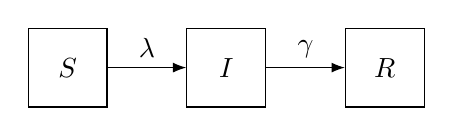
\begin{tikzpicture}[node distance=1cm, auto,
    >=Latex, 
    every node/.append style={align=center},
    int/.style={draw, minimum size=1cm}]
   \node [int] (S)             {$S$};
   \node [int, right=of S] (I) {$I$};
   \node [int, right=of I] (R) {$R$};
   \coordinate[right=of I] (out);
   \path[->] (S) edge node {$\lambda$} (I)
             (I) edge node {$\gamma$} (out);
\end{tikzpicture}
\end{figure}
\begin{equation}
  \frac{d S}{d t}=-\lambda S
  \label{eq:S_without_lockdown}
\end{equation}
\begin{equation}
  \frac{d I}{d t}=\lambda S-\gamma I
  \label{eq:I_without_lockdown}
\end{equation}
\begin{equation}
  \frac{d R}{d t}=\gamma I
  \label{eq:R_without_lockdown}
\end{equation}

Here, $\lambda$ is the force of infection, it is the rate at which susceptible individuals acquire an infectious disease~\cite{hens_aerts_faes_shkedy_lejeune_vandamme_beutels_2010}. It depends on other factors:

\begin{equation}
  \lambda = pc\frac{I}{N}
  \label{eq:lambda_force_of_infection}
\end{equation}

Here, 
$c$ is the average number of contacts a susceptible person makes per day.
$p$ is the probability of the susceptible person becomes infectious after coming into contact with an infectious person.
$\frac{I}{N}$ is the proportion of the contacts that are infectious.

And, $\beta$ the effective transmission rate is defined as:

\begin{equation}
  \beta = p c
  \label{eq:beta_effective_transmission_rate}
\end{equation}

During an epidemic, the fundamental drivers of an epidemic growth is the rate of infection $\beta$ i.e. the average number of infections per infected case and the infectious period $1/\gamma$ i.e. the average period for which the infected case is infected for. Epidemics can only happen if the case is infectious enough for long enough and this defined by $R_0 = \beta / \gamma$. Here, $R_0$ is The average number of secondary infections caused by each infected case, in an otherwise fully susceptible population.

At the peak of an epidemic $R_0$ declines as there are no more susceptible people left in the pool, therefore, $R_{eff}$ (effective reproductive number) comes into play. $R_{eff}$ is defined as the average number of secondary cases arising from an infected case, at a given point in an epidemic - therefore, it takes into account the existing immunity of the system. 

\begin{equation}
  R_{eff} = R_0 \frac{S}{N}
  \label{eq:R_effective}
\end{equation}

$S$ is the number of susceptible people, $N$ is the total population. At the start of an epidemic when everyone is susceptible, $R_{eff} = R_0$ as, $S = N$ (i.e. the whole population is susceptible). $\beta$ and $\gamma$ are also used to define probability of and infectious individual infecting another individual $\beta / (\beta + \gamma)$ and the probability of recovery, $\gamma / (\beta + \gamma)$.

Most government policies look at the value of $R_{eff}$ to come us with an effective strategy to combat the disease as the fate of the evolution of the disease depends upon it. When $R_{eff}$ is less than one, the infected population $I$ will steadily decline to zero. Conversely, if $R_{eff}$ is greater than one, the infected population will increase. In other words, when $\frac{dI(t)}{dt} < 0 \Rightarrow R_{eff} < 1$ and $\frac{dI(t)}{dt} > 0 \Rightarrow R_{eff} > 1},$ the effective reproductive rate $R_{eff}$ serves as a critical threshold that determines whether an infectious disease will rapidly extinguish or escalate into an epidemic~\cite{Cooper2020}.

To estimate the parameters $\beta$ and $\gamma$ for India, based on the data from May, 2020, to October, 2022, we simply define the cost to calibrate the model using the huber loss~\cite{huberloss}:

\begin{equation}
  L_{\delta}(y, f(x)) = 
  \begin{cases}
    \frac{1}{2}{(y - f(x))^2} & \text{for } |y - f(x)| \leq \delta, \\
    \delta \cdot (|y - f(x)| - \frac{1}{2}\delta) & \text{otherwise.}
  \label{eq:huberloss}
  \end{cases}
\end{equation}
\begin{equation}
  cost = L_{\delta = 1}(S, \hat{S}) + L_{\delta = 1}(I, \hat{I}) + L_{\delta = 1}(R, \hat{R})
  \label{eq:cost_SIR_model}
\end{equation}

Where, $S$ is the number of susceptible people and $\hat{S}$ is the predicted number of susceptible people, similarly, $I$ for infected and $\hat{I}$ for the predicted number of infected people, and $R$ for recovered. Minimizing this cost function using the Nelder-Mead method\cite{Gao2010}, we get:

\begin{equation}
  \beta_{optimal} = 0.04208479828695971
  \label{eq:beta_optimal_without_lockdown}
\end{equation}
\begin{equation}
  \gamma_{optimal} = 0.02388356686032017
  \label{eq:gamma_optimal_without_lockdown}
\end{equation}
\begin{equation}
  R_{0_{optimal}} = \frac{\beta_{optimal}}{\gamma_{optimal}} = 1.7620817917644795
  \label{eq:r0_without_lockdown}
\end{equation}
\begin{equation}
  cost = L_{\delta = 1}(S, \hat{S}) + L_{\delta = 1}(I, \hat{I}) + L_{\delta = 1}(R, \hat{R}) = 85051490.53250012
  \label{eq:cost_without_lockdown}
\end{equation}
See figure \ref{fig:SIR_model_IND} to see how the model compares with the real data.

Now that, we have a model -- we want to say $\beta$ is a time-varying parameter controlled by the stringency index, $s$~\cite{SIRLockdown,SIRLockdown2,analytical_covid_lockdown_model}. The stringency index is a composite measure based on nine response indicators including school closures, workplace closures, and travel bans, rescaled to a value from 0 to 100 (100 = strictest)~\cite{owidcoronavirus}. This index simply records the strictness of government policies and does not measure or imply the appropriateness or effectiveness of a country's response i.e. a higher score does not necessarily mean that a country's response is "better" than others lower on the index. 

To define the new time-varying beta that is dependent on the current stringency index, we say, 

\begin{equation}
  \frac{dS}{dt} = -\beta (1 - (s(t)/100)) \frac{S I}{N}
  \label{eq:S_with_lockdown}
\end{equation}
\begin{equation}
  \frac{dI}{dt} = \beta (1 - (s(t)/100)) \frac{S I}{N} - \gamma I
  \label{eq:I_with_lockdown}
\end{equation}
\begin{equation}
  \frac{dR}{dt} = \gamma I
  \label{eq:R_with_lockdown}
\end{equation}

Where, $s(t)$ is the stringency index at time $t$ and is scaled down by a factor of 100 to normalize it and bring it in the range $[0, 1]$. Optimizing this using the Nelder-Mead method we get:

\begin{equation}
  \beta_{optimal} = 0.4013340889432941
  \label{eq:beta_optimal_with_lockdown}
\end{equation}
\begin{equation}
  \gamma_{optimal} = 0.09017476605499258
  \label{eq:gamma_optimal_with_lockdown}
\end{equation}
\begin{equation}
  R_{0_{optimal}} = \frac{\beta_{optimal}}{\gamma_{optimal}} = 4.450625230328213
  \label{eq:r0_with_lockdown}
\end{equation}
\begin{equation}
  cost = L_{\delta = 1}(S, \hat{S}) + L_{\delta = 1}(I, \hat{I}) + L_{\delta = 1}(R, \hat{R}) = 98438821.45587364
  \label{eq:cost_with_lockdown}
\end{equation}

Finally, an additional flow from the susceptible population to the can be shown by adding a vaccination rate $\nu$ in the model. 

\begin{equation}
  \frac{dS}{dt} = -\beta (1 - (s(t)/100)) \frac{S I}{N} - \nu S
  \label{eq:S_with_lockdown_and_nu}
\end{equation}
\begin{equation}
  \frac{dI}{dt} = \beta (1 - (s(t)/100)) \frac{S I}{N} - \gamma I
  \label{eq:I_with_lockdown_and_nu}
\end{equation}
\begin{equation}
  \frac{dR}{dt} = \gamma I + \nu S
  \label{eq:R_with_lockdown_and_nu}
\end{equation}

Optimizing these equations with the Nelder-Mead method we get:

\begin{equation}
  \beta_{optimal} = 0.40897034072952304
  \label{eq:beta_optimal_with_lockdown_and_nu}
\end{equation}
\begin{equation}
  \gamma_{optimal} = 0.09196829370123338
  \label{eq:gamma_optimal_with_lockdown_and_nu}
\end{equation}
\begin{equation}
  \nu_{optimal} = 2.9044029843851936e-05
  \label{eq:nu_optimal_with_lockdown_and_nu}
\end{equation}
\begin{equation}
  R_{0_{optimal}} = \frac{\beta_{optimal}}{\gamma_{optimal}} = 4.446862329077204
  \label{eq:r0_with_lockdown_and_nu}
\end{equation}
\begin{equation}
  cost = L_{\delta = 1}(S, \hat{S}) + L_{\delta = 1}(I, \hat{I}) + L_{\delta = 1}(R, \hat{R}) = 94636860.38436058
  \label{eq:cost_with_lockdown_and_nu}
\end{equation}

However, as observed by the value of $\nu_{optimal}$ from \ref{eq:nu_optimal_with_lockdown_and_nu} which is almost negligible (close to zero) and the overestimation of infected individuals in \ref{fig:SIRV_model_with_lockdown_infections_IND} suggests that $\nu$ might be varying with time. This suggests a time-varying vaccination rate, wherein the transition from susceptibility to direct recovery fluctuates with time. Therefore, using the $\beta_{optimal}$ and $\gamma_{optimal}$ from \ref{eq:beta_optimal_with_lockdown_and_nu} and \ref{eq:gamma_optimal_with_lockdown_and_nu}, we optimize the value of $\nu$ given a sub-interval of $[{start}, {start} + {window}]$ where the ${window} = 20$ \cite{Marinov2022}. Here, ${window}$ is a hyperparameter that can be changed so as to reduce the cost function.

\begin{equation}
  \frac{dS}{dt} = -\beta_{optimal}  (1 - (s(t)/100))  \frac{S I}{N} - \nu S
  \label{eq:S_with_lockdown_and_nu_calc_nu}
\end{equation}
\begin{equation}
  \frac{dI}{dt} = \beta_{optimal}  (1 - (s(t)/100)) \frac{S I}{N} - \gamma_{optimal} I
  \label{eq:I_with_lockdown_and_nu_calc_nu}
\end{equation}
\begin{equation}
  \frac{dR}{dt} = \gamma_{optimal} I + \nu S
  \label{eq:R_with_lockdown_and_nu_calc_nu}
\end{equation}

This model gives us how $\nu$ varies with time.

\begin{figure}[H]
  \centering
  \caption{$\nu$ Varying with Time}
  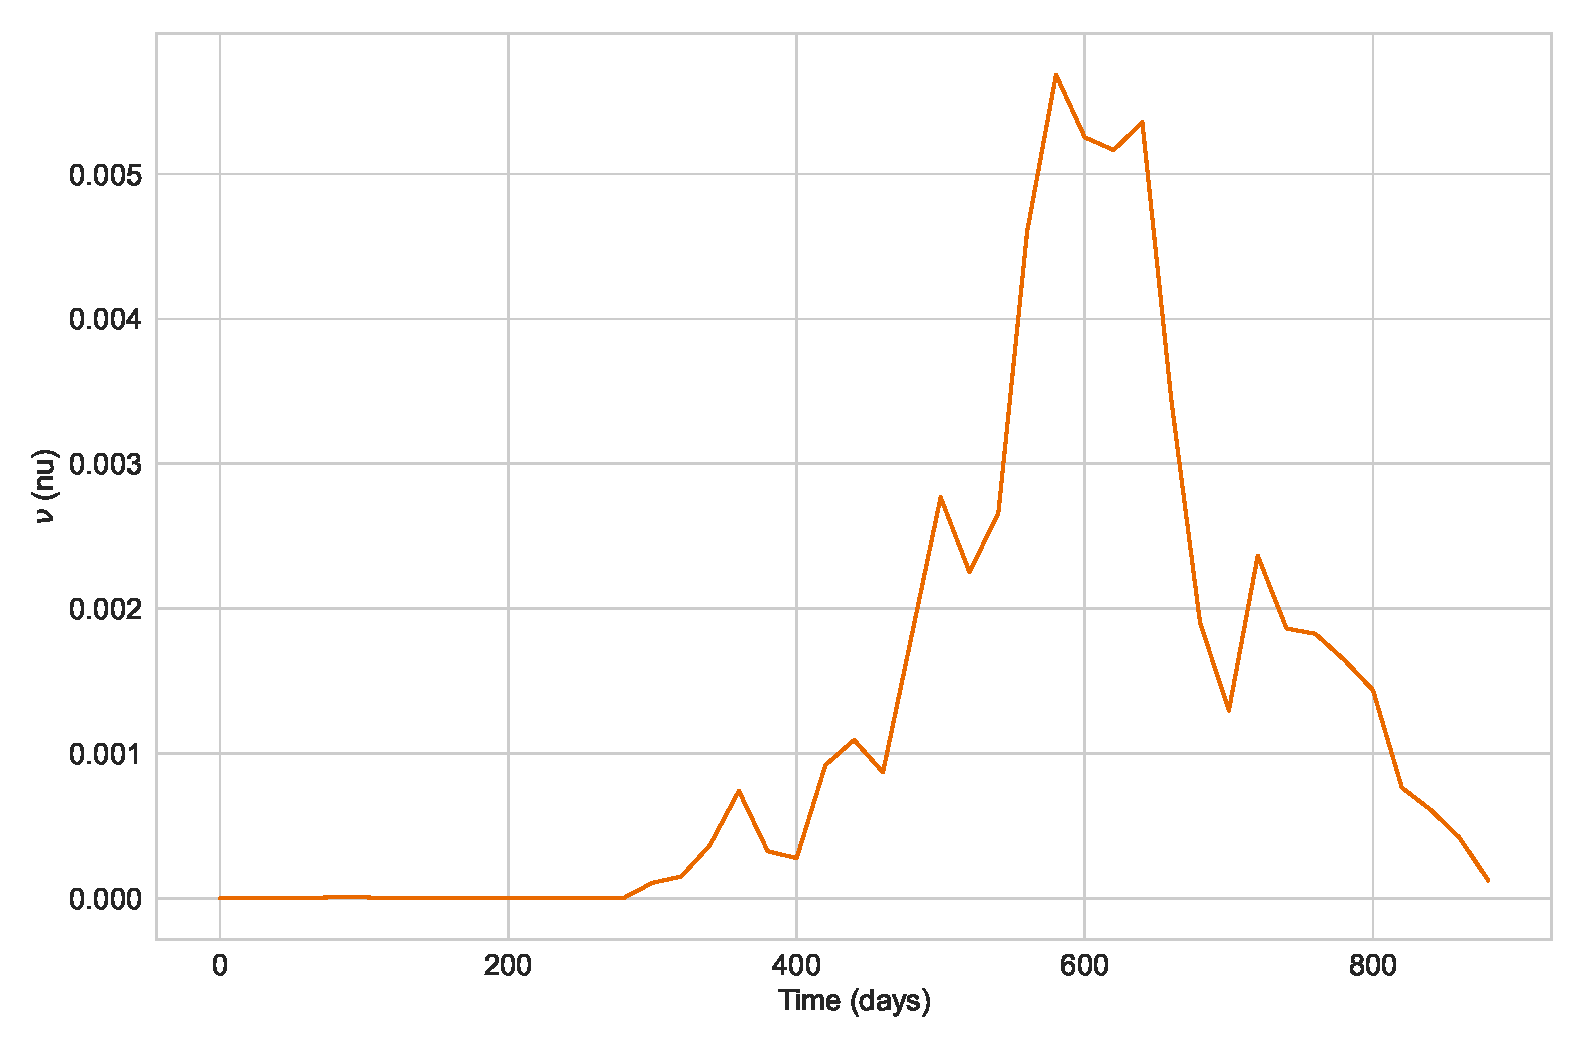
\includegraphics[width=\linewidth]{images/nu_varying_with_time_IND.eps}
  \label{fig:nu_varying_with_time_IND}
\end{figure}

Therefore, using these values we finally, recompute $\beta_{optimal}$ and $\gamma_{optimal}$ by supplying them into the equations below:

\begin{figure}[H]
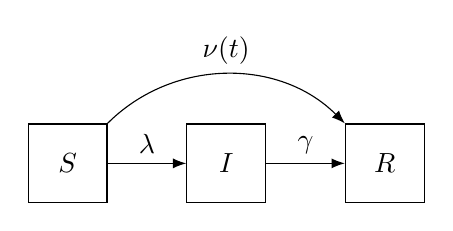
\begin{tikzpicture}[node distance=1cm, auto,
  >=Latex, 
  every node/.append style={align=center},
  int/.style={draw, minimum size=1cm}]
 \node [int] (S)             {$S$};
 \node [int, right=of S] (I) {$I$};
 \node [int, right=of I] (R) {$R$};
 \coordinate[right=of I] (out);
 \path[->] (S) edge node {$\lambda$} (I)
           (I) edge node {$\gamma$} (out)
           (S) edge[bend left=45] node[above] {$\nu(t)$} (R); % Arrow from S to R with text \nu(t)
\end{tikzpicture}
\end{figure}

\begin{equation}
  \frac{dS}{dt} = -\beta  (1 - (s(t)/100))  \frac{S I}{N} - \nu(t) S
  \label{eq:S_with_lockdown_and_time_varying_nu}
\end{equation}
\begin{equation}
  \frac{dI}{dt} = \beta  (1 - (s(t)/100)) \frac{S I}{N} - \gamma I
  \label{eq:I_with_lockdown_and_time_varying_nu}
\end{equation}
\begin{equation}
  \frac{dR}{dt} = \gamma I + \nu(t) S
  \label{eq:R_with_lockdown_and_time_varying_nu}
\end{equation}
\begin{equation}
  \beta_{optimal} = 0.5129414911377119
  \label{eq:beta_optimal_with_lockdown_and_time_varying_nu}
\end{equation}
\begin{equation}
  \gamma_{optimal} = 0.12716245167626106
  \label{eq:gamma_optimal_with_lockdown_and_time_varying_nu}
\end{equation}
\begin{equation}
  R_{0_{optimal}} = \frac{\beta_{optimal}}{\gamma_{optimal}} = 4.033749620081199
  \label{eq:r0_with_lockdown_and_time_varying_nu}
\end{equation}
\begin{equation}
  cost = L_{\delta = 1}(S, \hat{S}) + L_{\delta = 1}(I, \hat{I}) + L_{\delta = 1}(R, \hat{R}) = 29742589.698910963
  \label{eq:cost_with_lockdown_and_time_varying_nu}
\end{equation}

See (\ref{fig:SIR_model_IND}, ~\ref{fig:comparing_costs_IND}) to see how the different models compare against each other.

Now, that we have set up the following relation between $\beta$ and $s(t)$, we investigate how stringency index affects the normalized Gross domestic product (GDP). To do this we fit a polynomial equation of the third degree to the points $(x, y)$ where $x$ is the $s(t)$ stringency at time t, and $y$ the normalized GDP and minimize the squared error. For India after fitting a 3 degree polynomial we get the following equation:

\begin{equation}
    \begin{split}
      GDP = -5.96640236e-05 s^{3} + 6.65064332e-03 s^{2} -2.23109924e-01 s^{1} \\
    + 1.01357226e+02
    \end{split}
    \label{eq:gdp_modelled_with_stringency_IND}
\end{equation}

Given that the government is an agent that takes decisions in a deterministic environment defined above, we use reinforcement learning to model the competing costs of the environment. This environment is formally as a Markov decision process, and can be described as follows:
\begin{itemize}
    % \item \url{https://jmlr.org/papers/volume22/20-1364/20-1364.pdf} RL Paper that references \url{https://araffin.github.io/slides/rl-tuto-jnrr19/#/13} RL ppt (for our RL notes).
    \item Set of States $\altmathcal{S}$: The state of the environment are described through the descriptors like the normalized GDP ($(GDP_{predicted} - GDP_{min}) / (GDP_{max} - GDP_{min})$), $R_{eff}$, a list of all the previous actions (in changing the stringency) and the proportion of the population that was susceptible, infected and recovered. The starting states are simply these values at the starting date and no previous actions.
    \item TODO: FIX BELOW ITEM AFTER MODEL RUNS
    \item Actions $\altmathcal{A}$: The stringency index variable was analyzed with a sample size of 1034. The mean value was approximately 59.62, with a standard deviation of 22.82. The minimum value was 0, while the maximum value reached 100. And the differences between two consecutive stringencies had a mean of 0.030474, and standard deviation of 2.387331, with the minimum being -14.360000 and maximum 55.560000. Based on this we define the discrete action space. There are 7 actions for the agent, it can keep the stringency index same, reduce/increase by 2.5, reduce/increase by 5, and reduce/increase by 10 given that the stringency index doesn't exceed 100 or go below 0.
    \item Transition dynamics $\altmathcal{T}\left(\mathbf{s}_{t+1} \mid \mathbf{s}_t, \mathbf{a}_t\right)$ that map a state-action pair at time $t$ onto a distribution of states at time $t+1$. This state transition is defined by the SIR model with lockdown and the model of how stringency index affects the GDP.
    \item Immediate reward $\altmathcal{R}\left(\mathbf{s}_t, \mathbf{a}_t, \mathbf{s}_{t+1}\right)$. Here we define a reward strategy however it should be noted that this strategy can be easily changed to prioritize different needs.
    \item Discount Factor $\gamma \in[0,1]$, where lower values place more emphasis on immediate rewards. Here, we choose the default discount factor of 0.99.
\end{itemize}
In general, the policy $\pi$ is a mapping from states to a probability distribution over actions: $\pi: \altmathcal{S} \rightarrow p(\altmathcal{A}=\mathbf{a} \mid \altmathcal{S})$. If the MDP is episodic, i.e., the state is reset after each episode of length $T$, then the sequence of states, actions and rewards in an episode constitutes a trajectory or rollout of the policy. Every rollout of a policy accumulates rewards from the environment, resulting in the return $R=\sum_{t=0}^{T-1} \gamma^t r_{t+1}$. The goal of RL is to find an optimal policy, $\pi^*$, which achieves the maximum expected return from all states.

The stringency index emerges as a critical factor influencing both the Gross Domestic Product (GDP) and the rate of infection spread. The decision to escalate or de-escalate the stringency index is a strategic one, with significant implications. Increasing the stringency decreases the spread of the infection. Conversely, it must be noted that herd immunity can only be achieved when the epidemic reaches its peak i.e. when the effective reproductive number is equal to one ($R_{eff} = 1$). This can only happen by lowering the stringency index which would allow the natural dynamics of the epidemic to transpire such that the population of susceptible individuals has depleted enough such that it is insufficient to propagate the disease further. Therefore, stringency is used to control the number of infected people and slow down the rate at which the epidemic reaches its peak, so that hospitals could house the number of infected people.

With this basis we define the reward function~\cite{Ohi2020}. In Deep Reinforcement Learning (DRL), positive rewards promote and negative rewards demote actions. The agent tries to generate such a policy/knowledge to avoid the discouraging situation by following the policy. By designing a proper reward function, it is possible to generate such an agent that may follow the human desired situation.

The reward function is parameterized to account for key factors influencing decision-making. To incentivize reduction of $R{eff}$ (effective reproductive number) a negative reward is imposed of $-20 * R_{eff}$, but as the $R_{eff}$ is between $[1.9, 1,5]$ we start to positively reward it with a multiple of the GDP ($100 * \textrm{min\_max\_normalized\_GDP}$) and if the $R_{eff}$ is below $1.5$ then $200 * \textrm{min\_max\_normalized\_GDP}$. Furthermore, there's a simple positive reward of $10$ if $R_{eff}$ is below the threshold value ($1.9$) and negative reward of $-10$ otherwise. To reward not changing the stringencies frequently, we reward the absolute different between the previous stringency and the current stringency negatively ($|s(t) - s(t-1)| * -1 * 5$) [TODO: this factor should be reduced back to 2 from 5]. If the proportion of the infected population were to rise above 0.003 the model is punished ($-5000$) and otherwise rewarded ($+20$). It should be realized there can be an infinite number of ways to design the reward function to be more human and upgrade the way a decision is taken given the situation \cite{AWSDeepRacer}. Therefore, this research act as a  framework for promoting the development of more efficient reward strategies for the same. 

The agent observes the percentage of the population that is susceptible, infected, recovered, and the GDP which extrapolated from the stringency index and all the past moves played, i.e., all the past stringency indexes decided by the agent. The following values are fed into a simple network. Stable Baselines3 supports multiple inputs by using Dict Gym space. This can be done using MultiInputPolicy, which by default uses the CombinedExtractor features extractor to turn multiple inputs into a single vector, handled by the network arch network.

For data that varies with time we use a simple LSTM architecture.

% we utilized a custom combined extractor, a unique type of Long Short-Term Memory (LSTM) network, for processing our data. This network was designed to handle different types of input data encapsulated in an observation space, which is a common concept in reinforcement learning representing the information an agent observes from the environment. The CustomCombinedExtractor class, which inherits from the BaseFeaturesExtractor class, was initialized with an observation space that is a dictionary of Gym spaces. The Gym spaces module provides a set of high-level, easy-to-use data structures for defining observation and action spaces, which are essential components in reinforcement learning. The extractor contains a dictionary of individual extractors for each key in the observation space. If the subspace shape is equal to the total number of days plus one, an LSTM extractor is created with an input size of 1 and a hidden size of 16. This LSTM extractor is designed to handle sequential data, which is particularly useful for time-series data such as ours. For the 'other_stats' key, a Flatten extractor is used to flatten the input data. In the forward method, the observations are processed through their respective extractors. For LSTM extractors, the final hidden state is used as the output. All the processed observations are then concatenated into a single tensor. The observation space for the deep learning type is defined as a dictionary of four keys: 'stringency', 'normalized_gdp', 'r_eff', and 'other_stats'. Each key is associated with a Box space, which is a multi-dimensional box that allows for a range of numerical values. The shape of the Box space defines the dimensionality of the data, and the low and high parameters define the range of possible values. This LSTM network and the associated observation space provide a robust framework for processing and learning from our complex, multi-dimensional data.

\newcommand{\DrawNeuronalNetwork}[2][]{
\xdef\Xmax{0}
\foreach \Layer/\X/\Col/\Miss/\Lab/\Count/\Content [count=\Y] in {#2}
{\pgfmathsetmacro{\Xmax}{max(\X,\Xmax)}
 \xdef\Xmax{\Xmax}
 \xdef\Ymax{\Y}
}
\foreach \Layer/\X/\Col/\Miss/\Lab/\Count/\Content [count=\Y] in {#2}
{\node[anchor=south] at ({2*\Y},{\Xmax/2+0.1}) {\Layer};
 \foreach \m in {1,...,\X}
 {
  \ifnum\m=\Miss
   \node [neuron missing] (neuron-\Y-\m) at ({2*\Y},{\X/2-\m}) {};
  \else
   \node [circle,fill=\Col!50,minimum size=1cm] (neuron-\Y-\m) at 
  ({2*\Y},{\X/2-\m}) {\Content};
 \ifnum\Y=1
  \else
   \pgfmathtruncatemacro{\LastY}{\Y-1}
   \foreach \Z in {1,...,\LastX}
   {
    \ifnum\Z=\LastMiss
    \else
     \draw[->] (neuron-\LastY-\Z) -- (neuron-\Y-\m);
    \fi
    }
  \fi
 \fi
 \ifnum\Y=1
  \ifnum\m=\X
   \draw [overlay] (neuron-\Y-\m) -- (state);
  \else
   \ifnum\m=\Miss
   \else
    \draw [overlay] (neuron-\Y-\m) -- (state);
   \fi
  \fi
 \else
 \fi     
 }
 \xdef\LastMiss{\Miss}
 \xdef\LastX{\X}
}
}
\begin{tikzpicture}[x=1.5cm, y=1.5cm,
>=stealth,font=\sffamily,nodes={align=center}]
 \begin{scope}[local bounding box=T]
  \path  node[draw,minimum width=6em,minimum height=4em] (state) {State};
  \begin{scope}[local bounding box=NN]
   \DrawNeuronalNetwork{Input Layer/5/green/4///,
     Hidden Layer/5/blue/4//11/,
     Output Layer/4/red/3//11/}
  \end{scope}
  \path (NN.south) node[below]{Estimated parameter\\ $\theta$};
  \path(NN.east) -- node[above]{Policy\\ $\Pi(\theta,a)$}++ (4em,0);
 \end{scope} 
 \node[fit=(T),label={[anchor=north west]north west:Agent},inner sep=1em,draw]
  (TF){};
 \node[below=3em of TF,draw,inner sep=1em] (Env) {Environment};
 \draw[<-] (TF.200) -- ++ (-1em,0) |- (Env.160) node[pos=0.45,right]{$r_t$};
 \draw[<-] (TF.180) -- ++ (-2em,0) |- (Env.180) node[pos=0.45,left]{$s_t$};
 \draw[->] (NN.east) -- ++ (7em,0)node[right]{$a_t$} |- (Env);
\end{tikzpicture}

% Use this for the RL formulae: https://arxiv.org/pdf/1708.05866.pdf and https://www.nature.com/articles/s41598-022-23668-x
% for reward function use this: https://www.nature.com/articles/s41598-020-79147-8

\subsection*{Results}
% https://www.nature.com/articles/s41598-020-79147-8 (see this to write results)
Using the simple SIR model (\ref{eq:S_without_lockdown}, ~\ref{eq:cost_without_lockdown}) to model the disease dynamics we get:
\begin{figure}[H]
  \centering
  \caption{SIR Model with lockdown for India}
  \begin{subfigure}[t]{\textwidth}
    \centering
    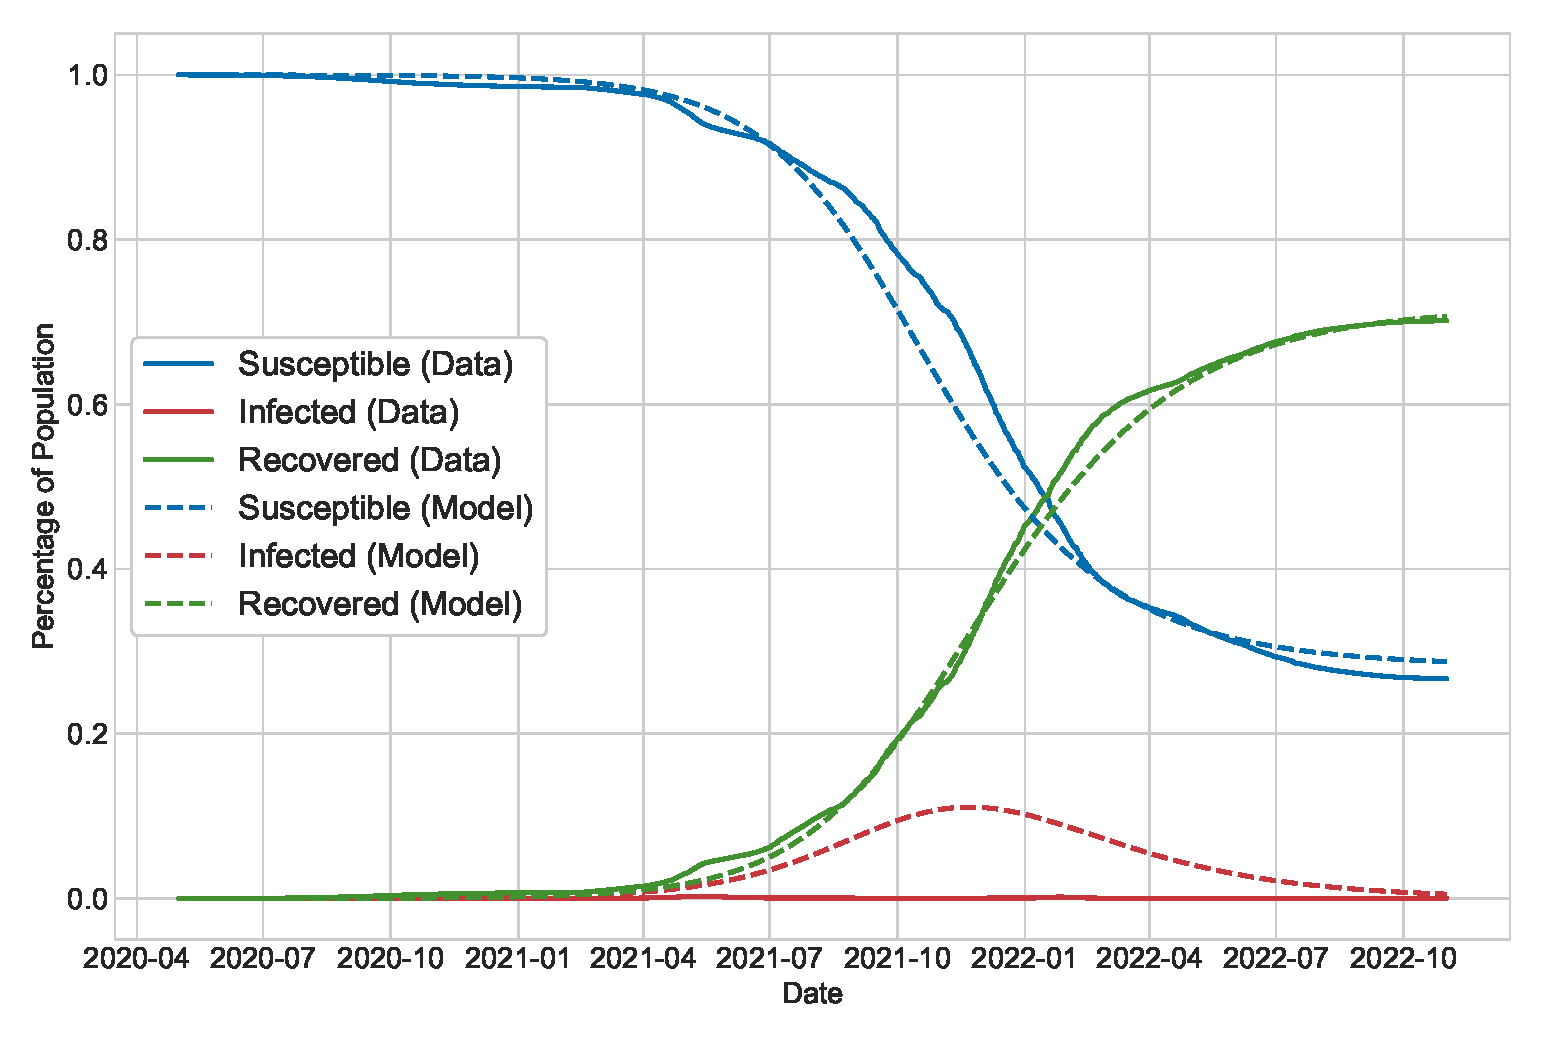
\includegraphics[scale=0.5]{images/SIR_model_IND.eps}
    \caption{SIR model with lockdown}
    \label{fig:SIR_model_IND}
  \end{subfigure}
  \begin{subfigure}[t]{\textwidth}
    \centering
    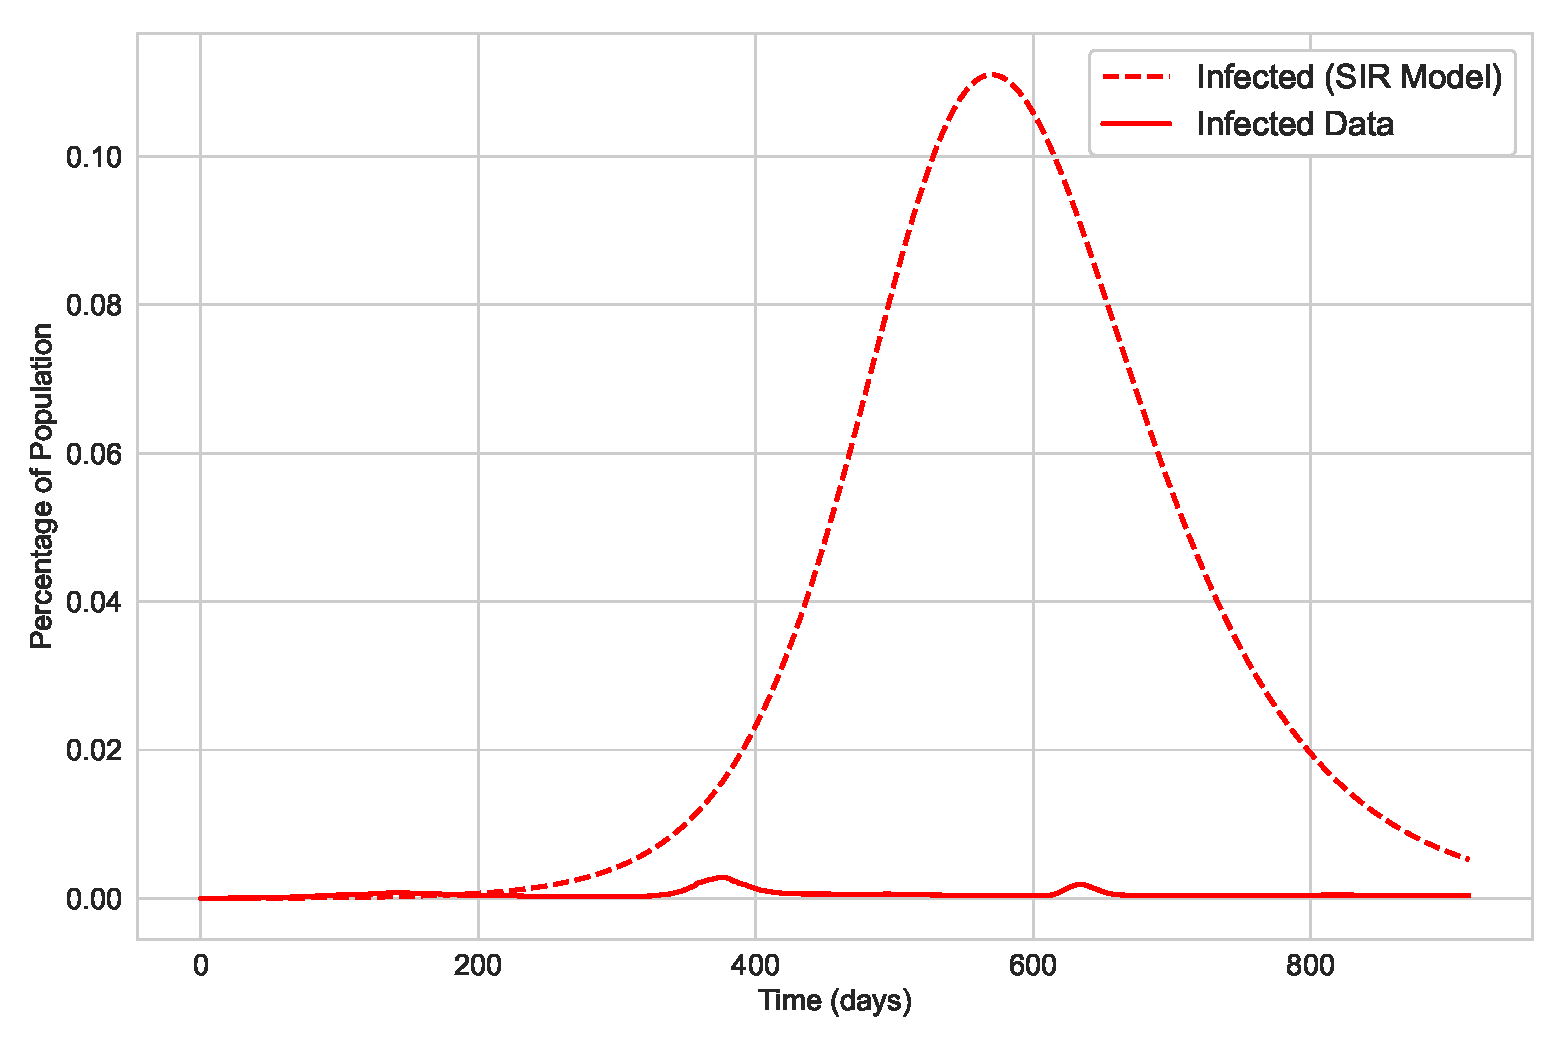
\includegraphics[scale=0.50]{images/SIR_model_infections_IND.eps}
    \caption{Infections modelled with SIR model}
    \label{fig:SIR_model_infections_IND}
  \end{subfigure}
\end{figure}
Here, it can be observed that the SIR model accurately fits the susceptible population and recovered population but overestimates the infected population by a significant margin. Although overestimating the infected population may not always be problematic, in our specific case, it can create complications. This is because our research involves rewarding the agent when the proportion of infected individuals falls below a predetermined threshold. Consequently, an overestimation of the infected population could lead to incorrect decision-making and undesirable outcomes.

Combining the lockdown dynamics in the SIR model (\ref{eq:S_with_lockdown}, ~\ref{eq:cost_with_lockdown}) we get the following:
\begin{figure}[H]
  \centering
  \caption{SIR Model with lockdown for India}

  \begin{subfigure}[t]{\textwidth}
    \centering
    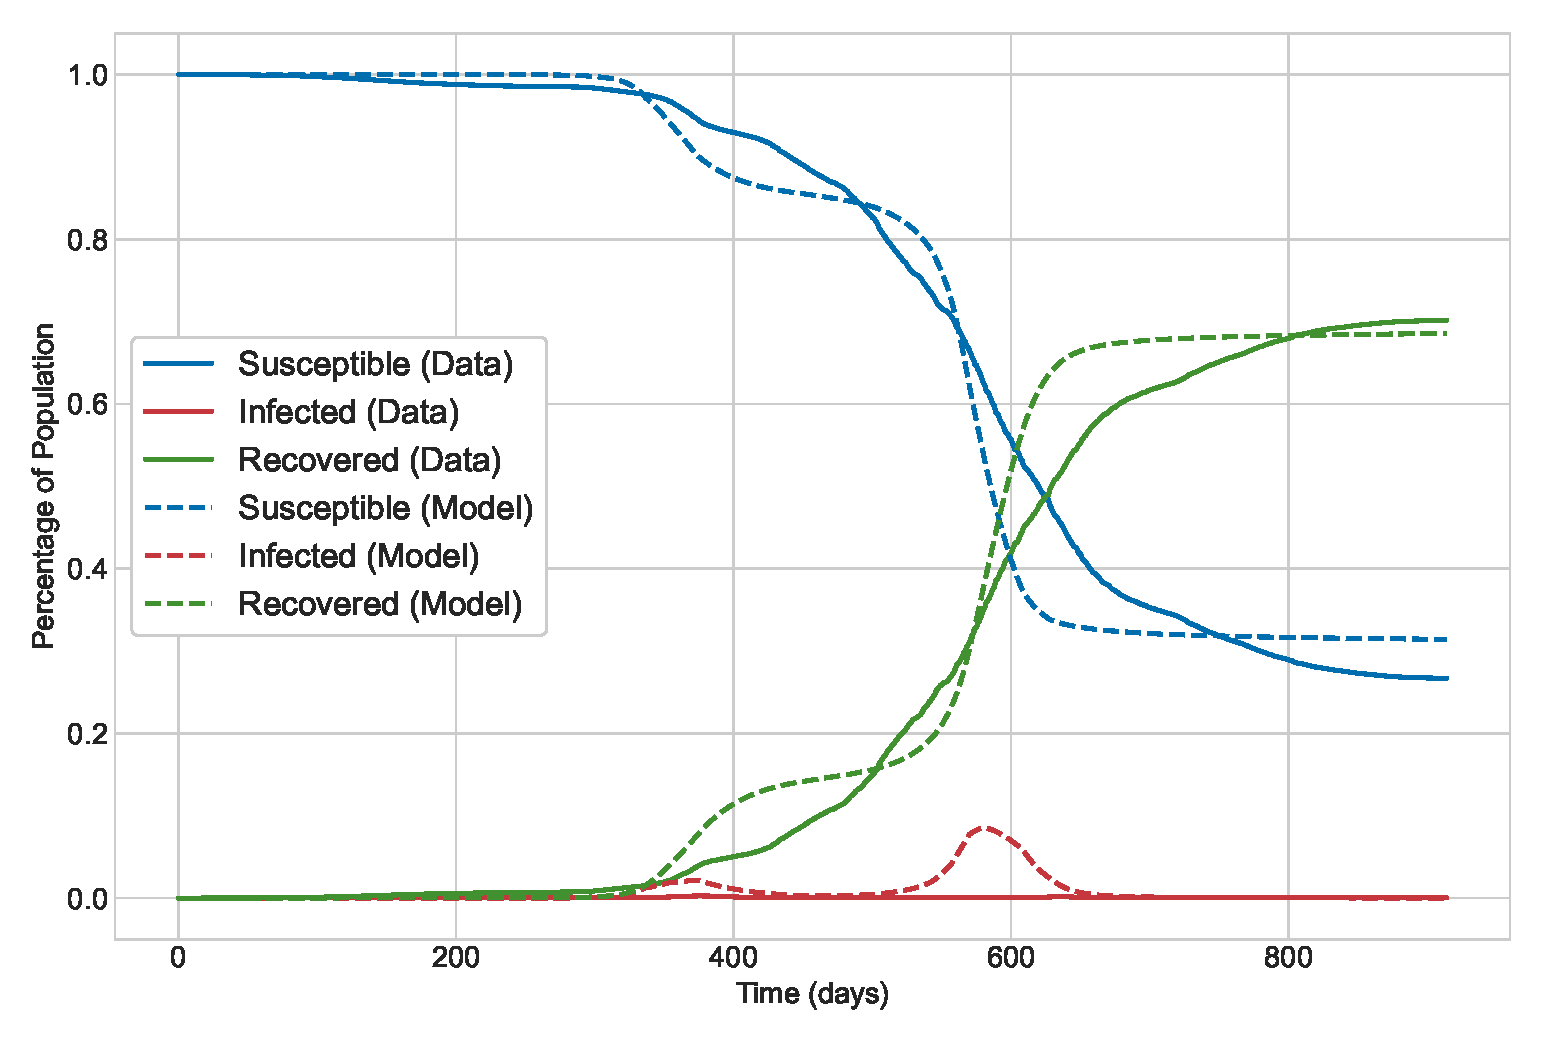
\includegraphics[scale=0.50]{images/SIR_model_with_lockdown_IND.eps}
    \caption{SIR model with lockdown}
    \label{fig:SIR_model_with_lockdown_IND}
  \end{subfigure}
  
  \begin{subfigure}[t]{\textwidth}
    \centering
    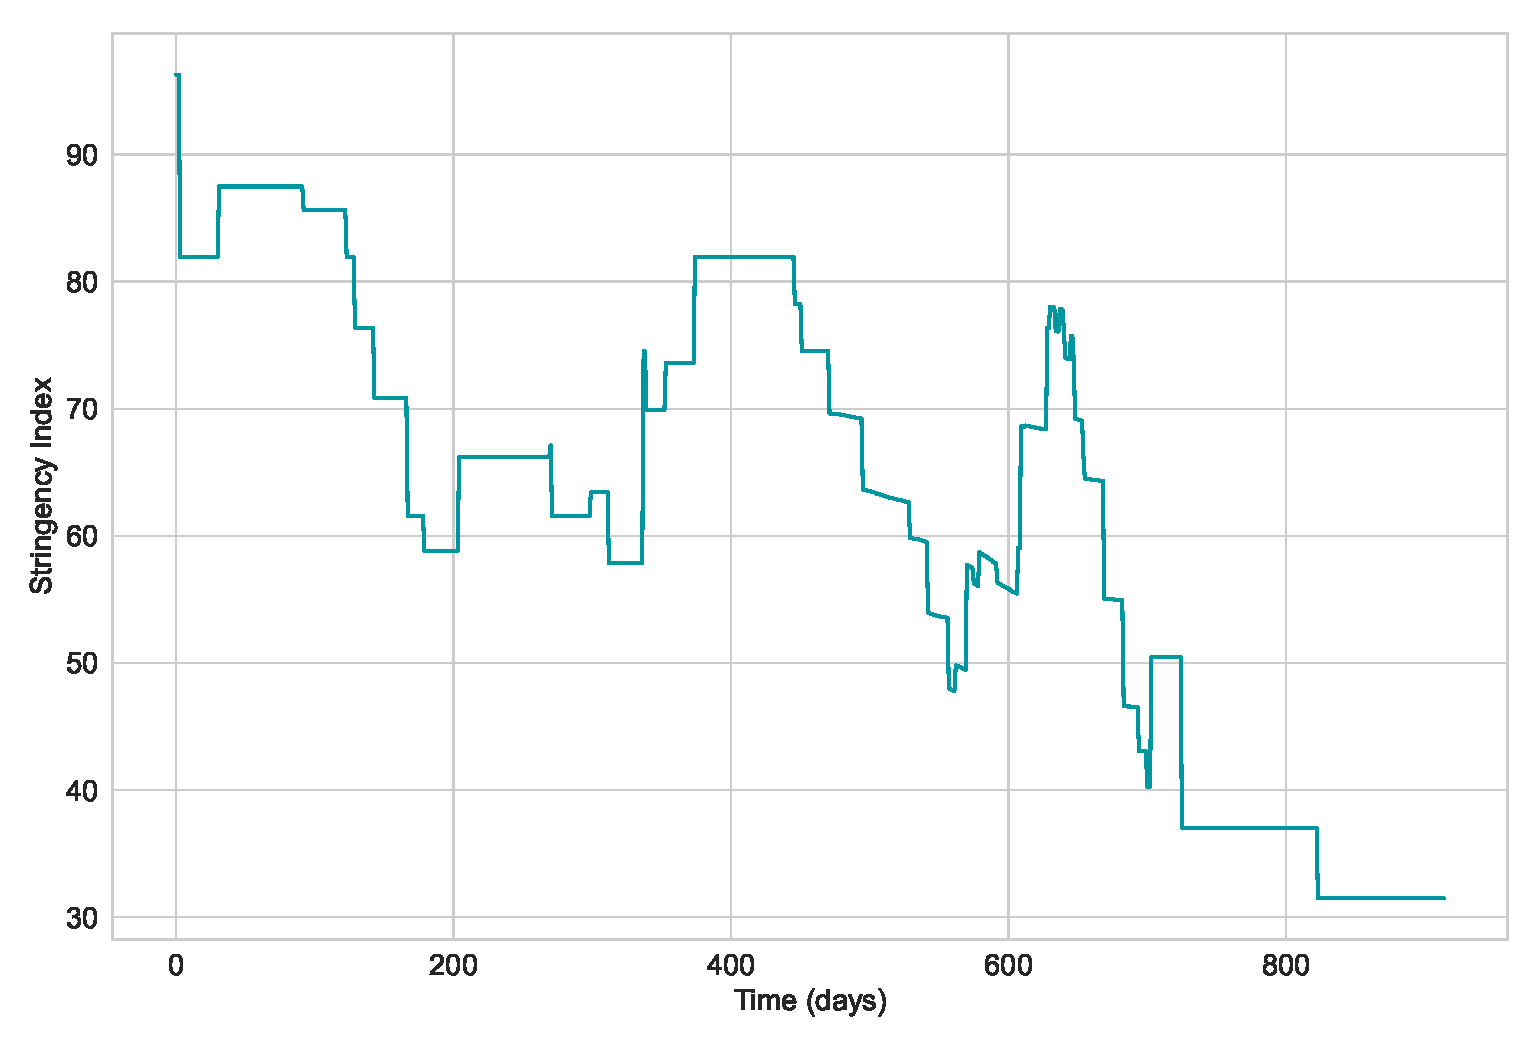
\includegraphics[scale=0.50]{images/stringency_varying_with_time_IND.eps}
    \caption{Stringency varying with Time}
    \label{fig:stringency_varying_with_time_IND}
  \end{subfigure}
\end{figure}
\begin{figure}[H]\ContinuedFloat
  \begin{subfigure}[t]{\textwidth}
    \centering
    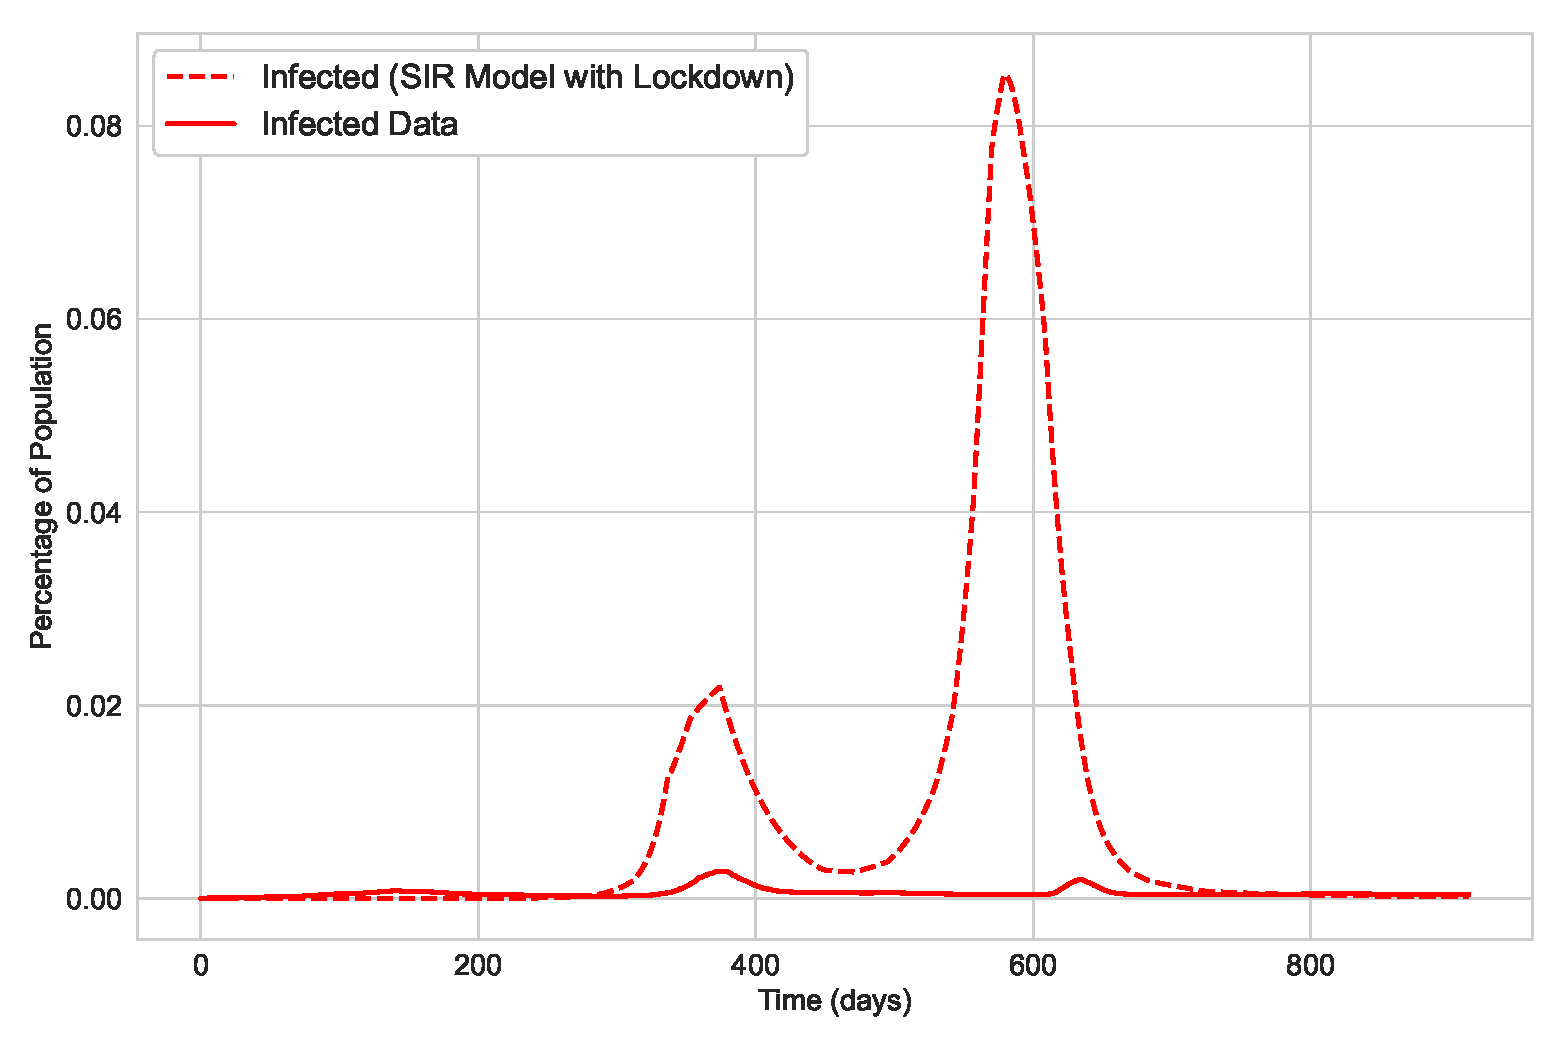
\includegraphics[scale=0.50]{images/SIR_model_with_lockdown_infections_IND.eps}
    \caption{Infections modelled with SIR model with Lockdown}
    \label{fig:SIR_model_with_lockdown_infections_IND}
  \end{subfigure}
\end{figure}
Here, it can be observed there's an overestimation of infected individuals, but, the two stages of the epidemic are being accounted for. This is what suggests that there might be depletion of infected individuals through vaccination.

Combining vaccination dynamics with SIR with lockdown model (\ref{eq:S_with_lockdown_and_nu}, ~\ref{eq:cost_with_lockdown_and_nu}) we get the following:
\begin{figure}[H]
  \centering
  \caption{SIRV Model with lockdown for India}

  \begin{subfigure}[t]{\textwidth}
    \centering
    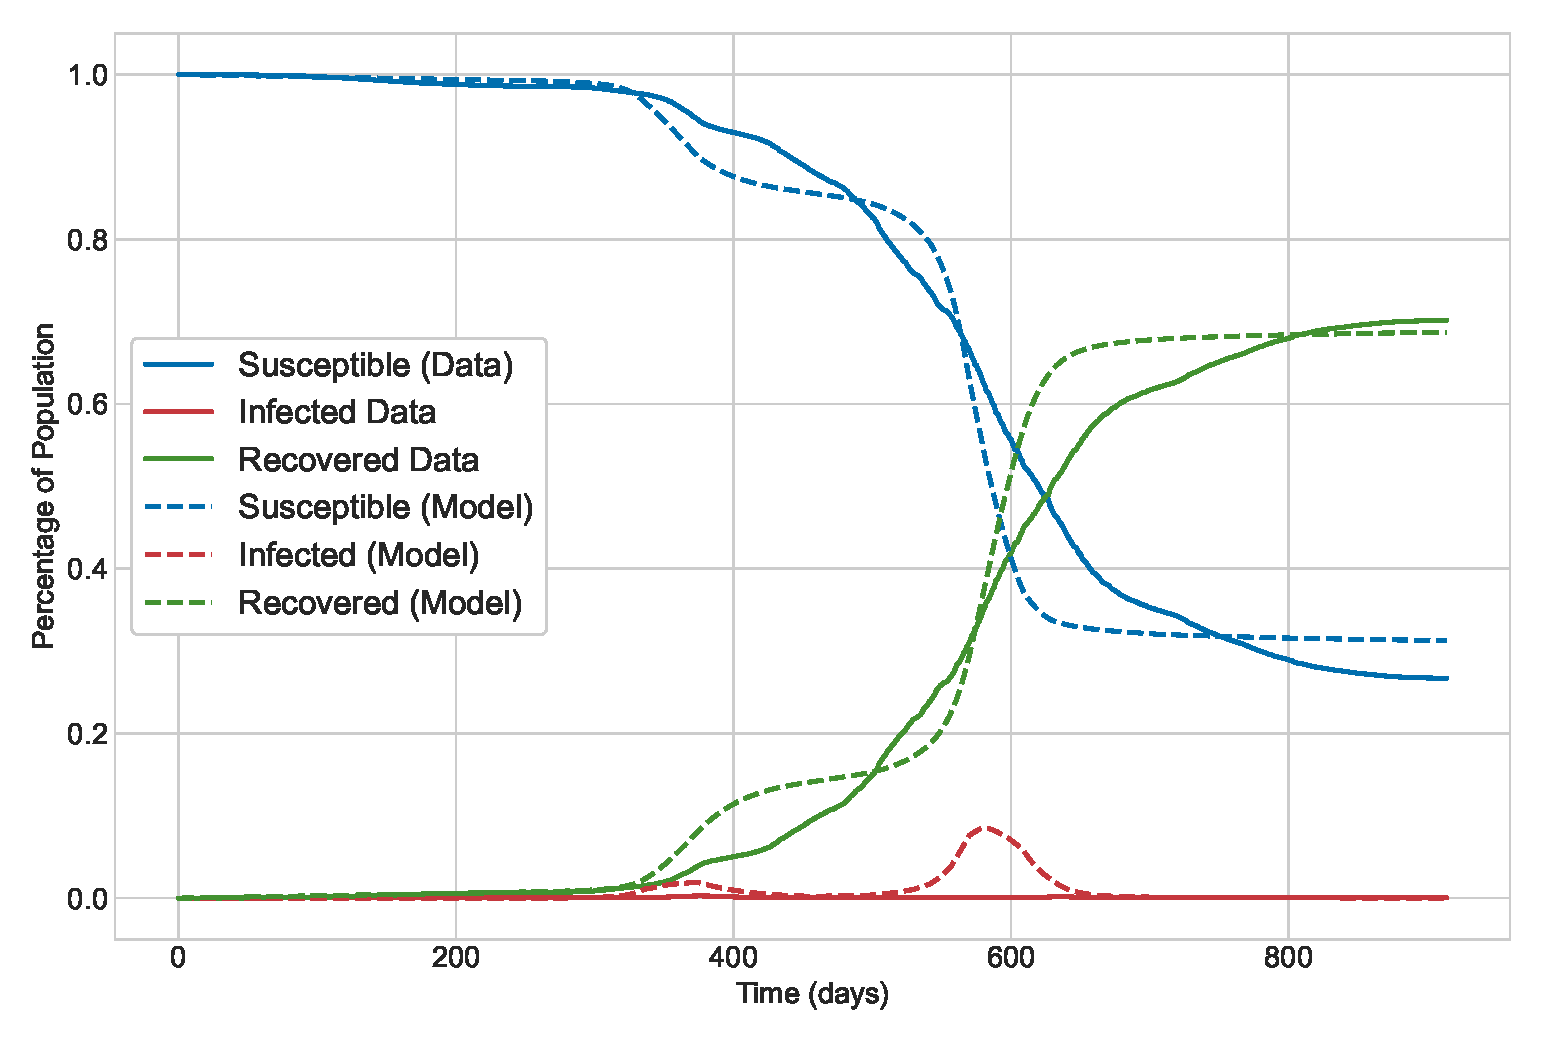
\includegraphics[scale=0.50]{images/SIRV_model_with_lockdown_IND.eps}
    \caption{SIRV model with lockdown}
    \label{fig:SIRV_model_with_lockdown_IND}
  \end{subfigure}

  \begin{subfigure}[t]{\textwidth}
    \centering
    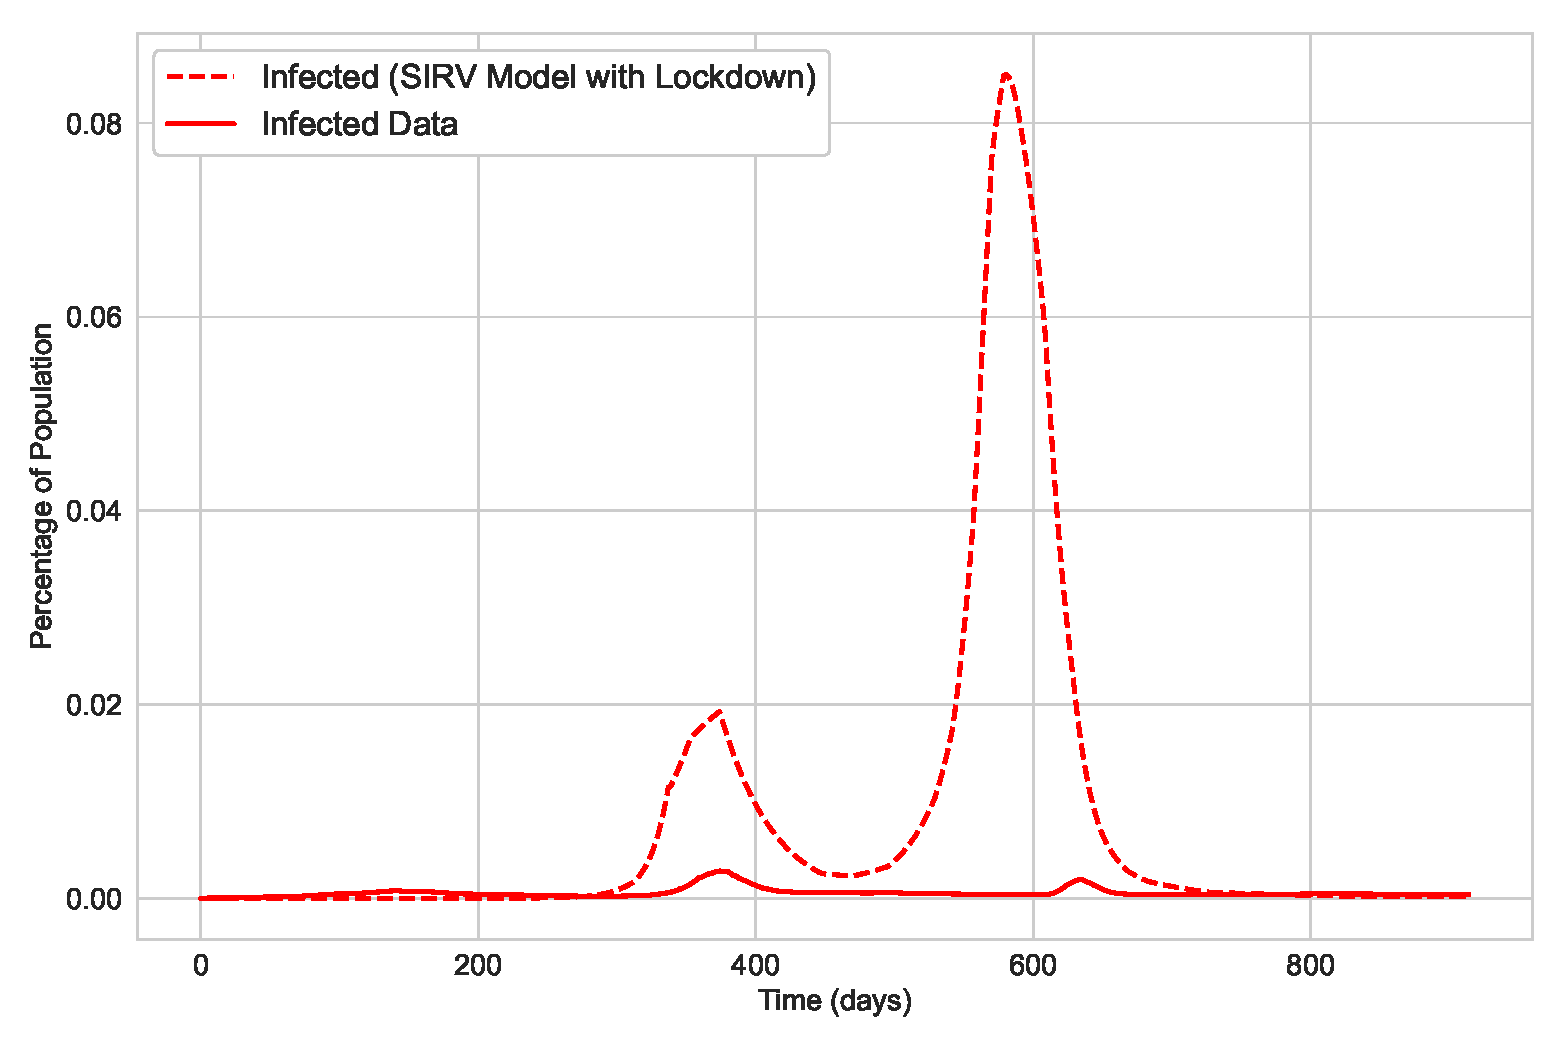
\includegraphics[scale=0.50]{images/SIRV_model_with_lockdown_infections_IND.eps}
    \caption{Infections modelled with SIRV model with Lockdown}
    \label{fig:SIRV_model_with_lockdown_infections_IND}
  \end{subfigure}

\end{figure}
Here, because the value of $\nu$ (\ref{eq:nu_optimal_with_lockdown_and_nu}) is negligible, it makes no change. However, time-varying $\nu$ shall be able to better account for the these dynamics.

For time-varying $\nu$ and SIRV model with lockdown (\ref{eq:S_with_lockdown_and_time_varying_nu}, ~\ref{eq:cost_with_lockdown_and_time_varying_nu}), we get the folllowing:
\begin{figure}[H]
  \centering
  \caption{SIRV Model with lockdown and time-varying $\nu$ for India}

  \begin{subfigure}[t]{\textwidth}
    \centering
    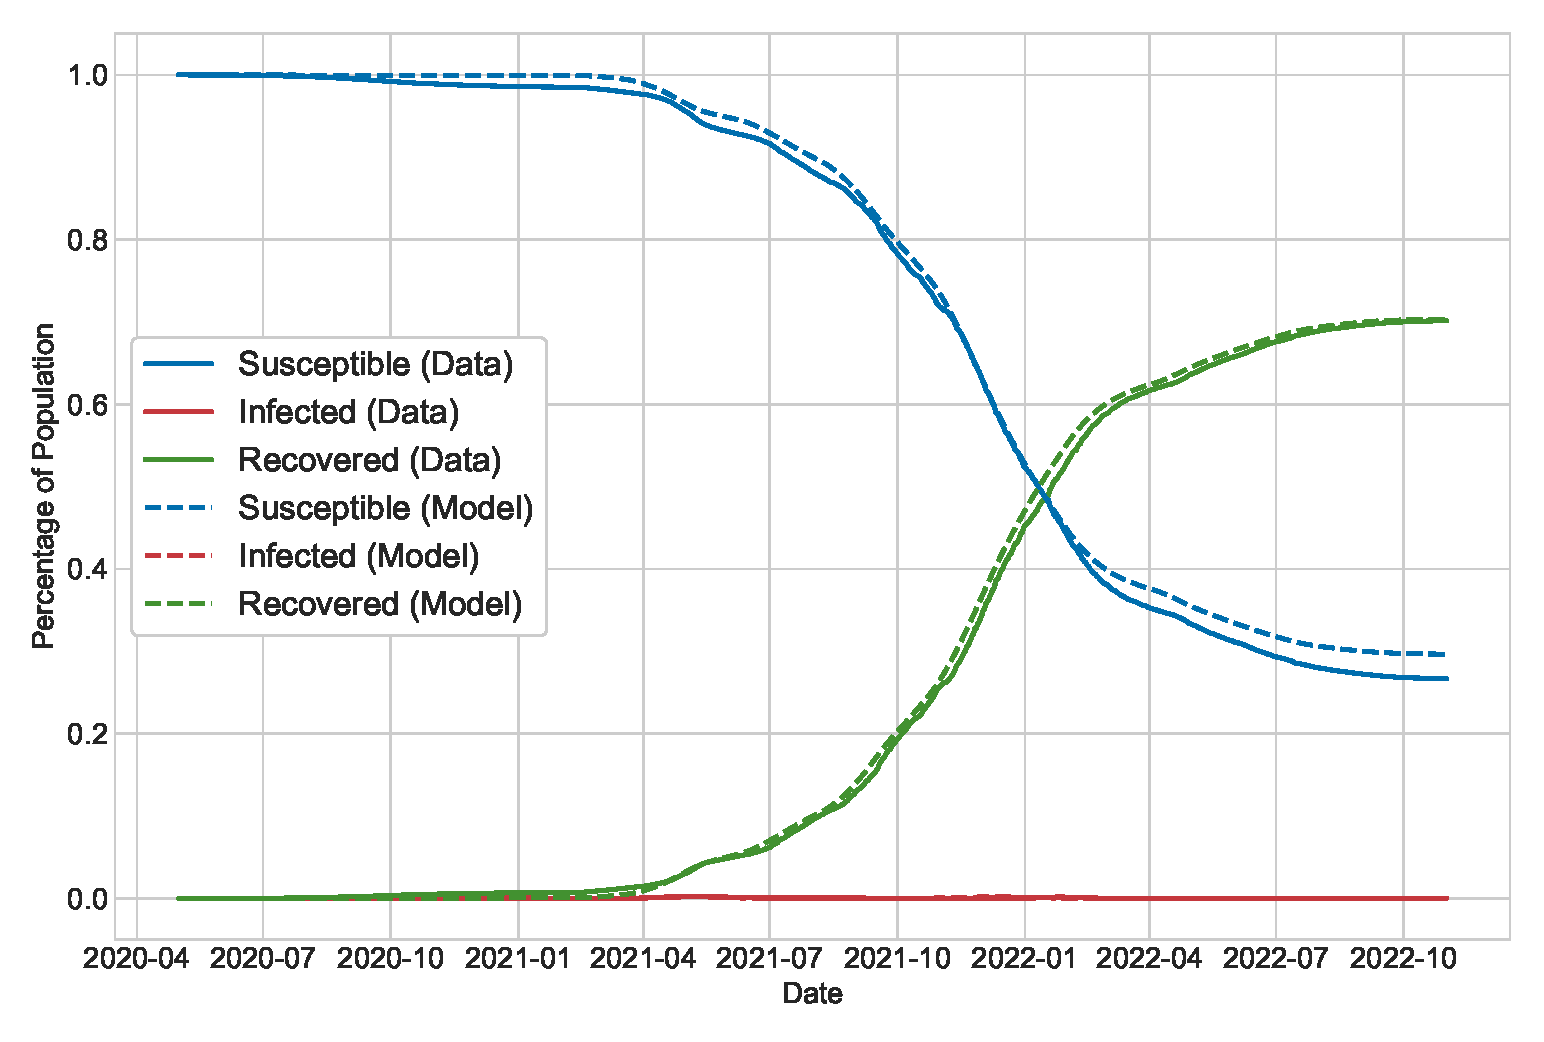
\includegraphics[scale=0.50]{images/SIRV_model_with_lockdown_time_varying_nu_IND.eps}
    \caption{SIRV model with lockdown and time-varying $\nu$}
    \label{fig:SIRV_model_with_lockdown_time_varying_nu_IND}
  \end{subfigure}

  \begin{subfigure}[t]{\textwidth}
    \centering
    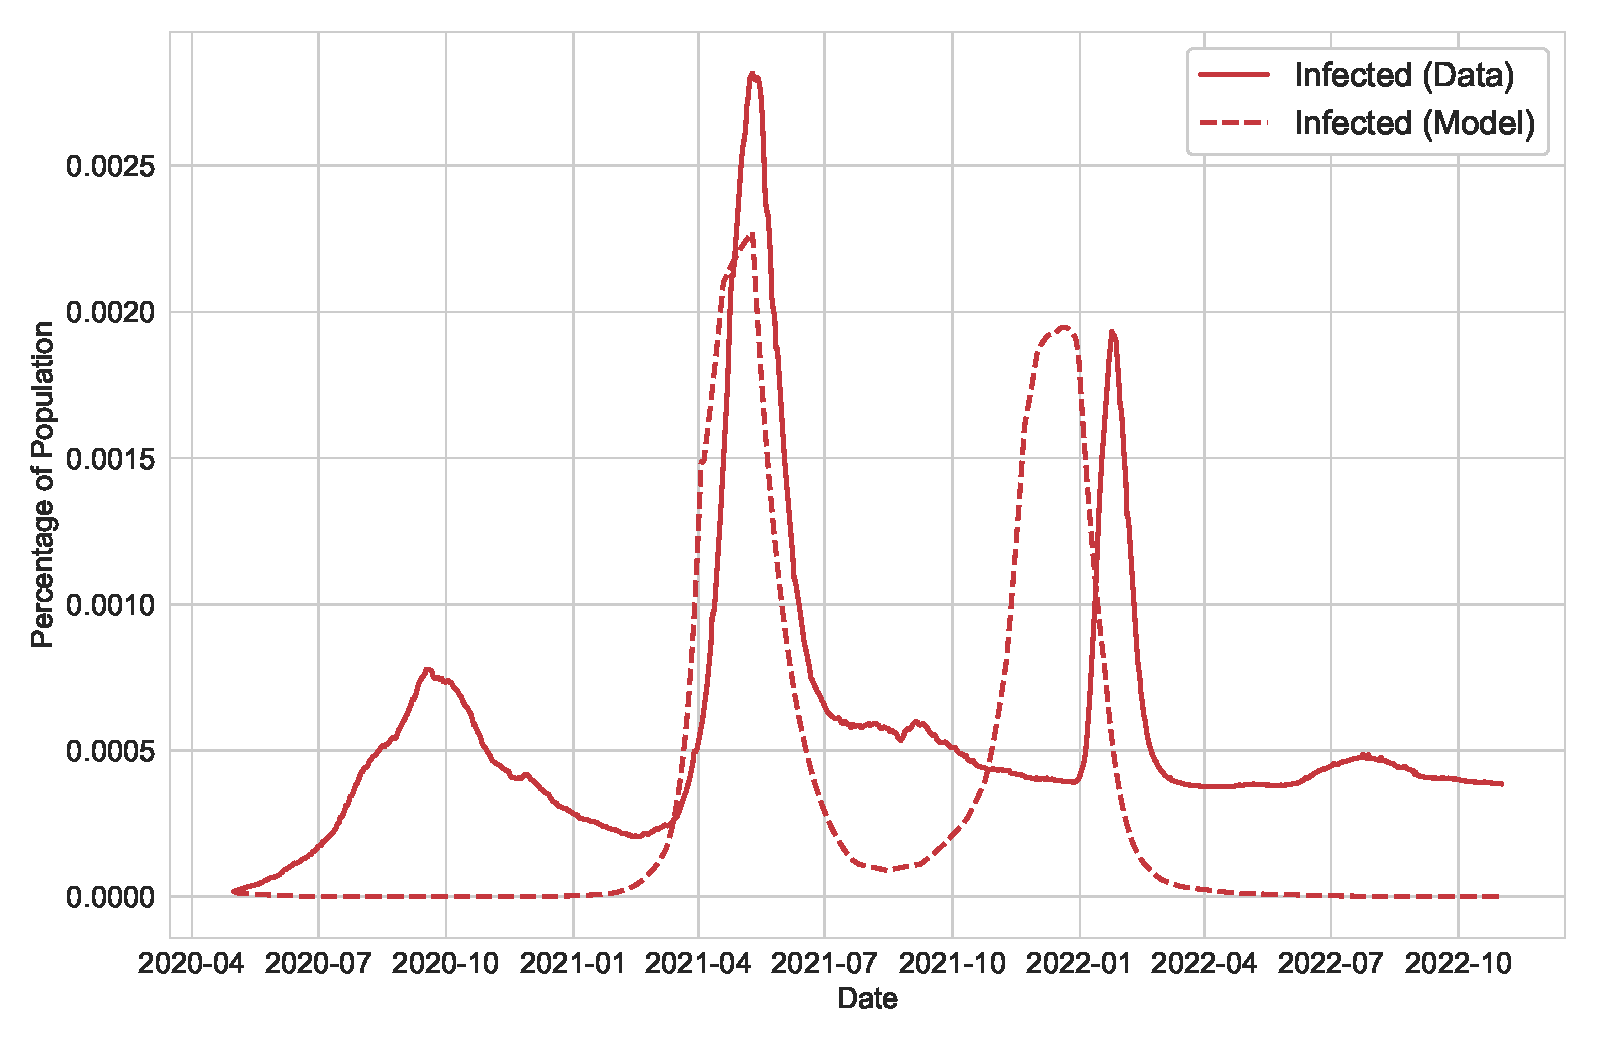
\includegraphics[scale=0.50]{images/SIRV_model_with_lockdown_infections_time_varying_nu_IND.eps}
    \caption{Infections modelled with SIRV model with Lockdown and time-varying $\nu$}
    \label{fig:SIRV_model_with_lockdown_infections_time_varying_nu_IND}
  \end{subfigure}
\end{figure}

\begin{figure}[H]
  \centering
  \caption{Loss for Different Models}
  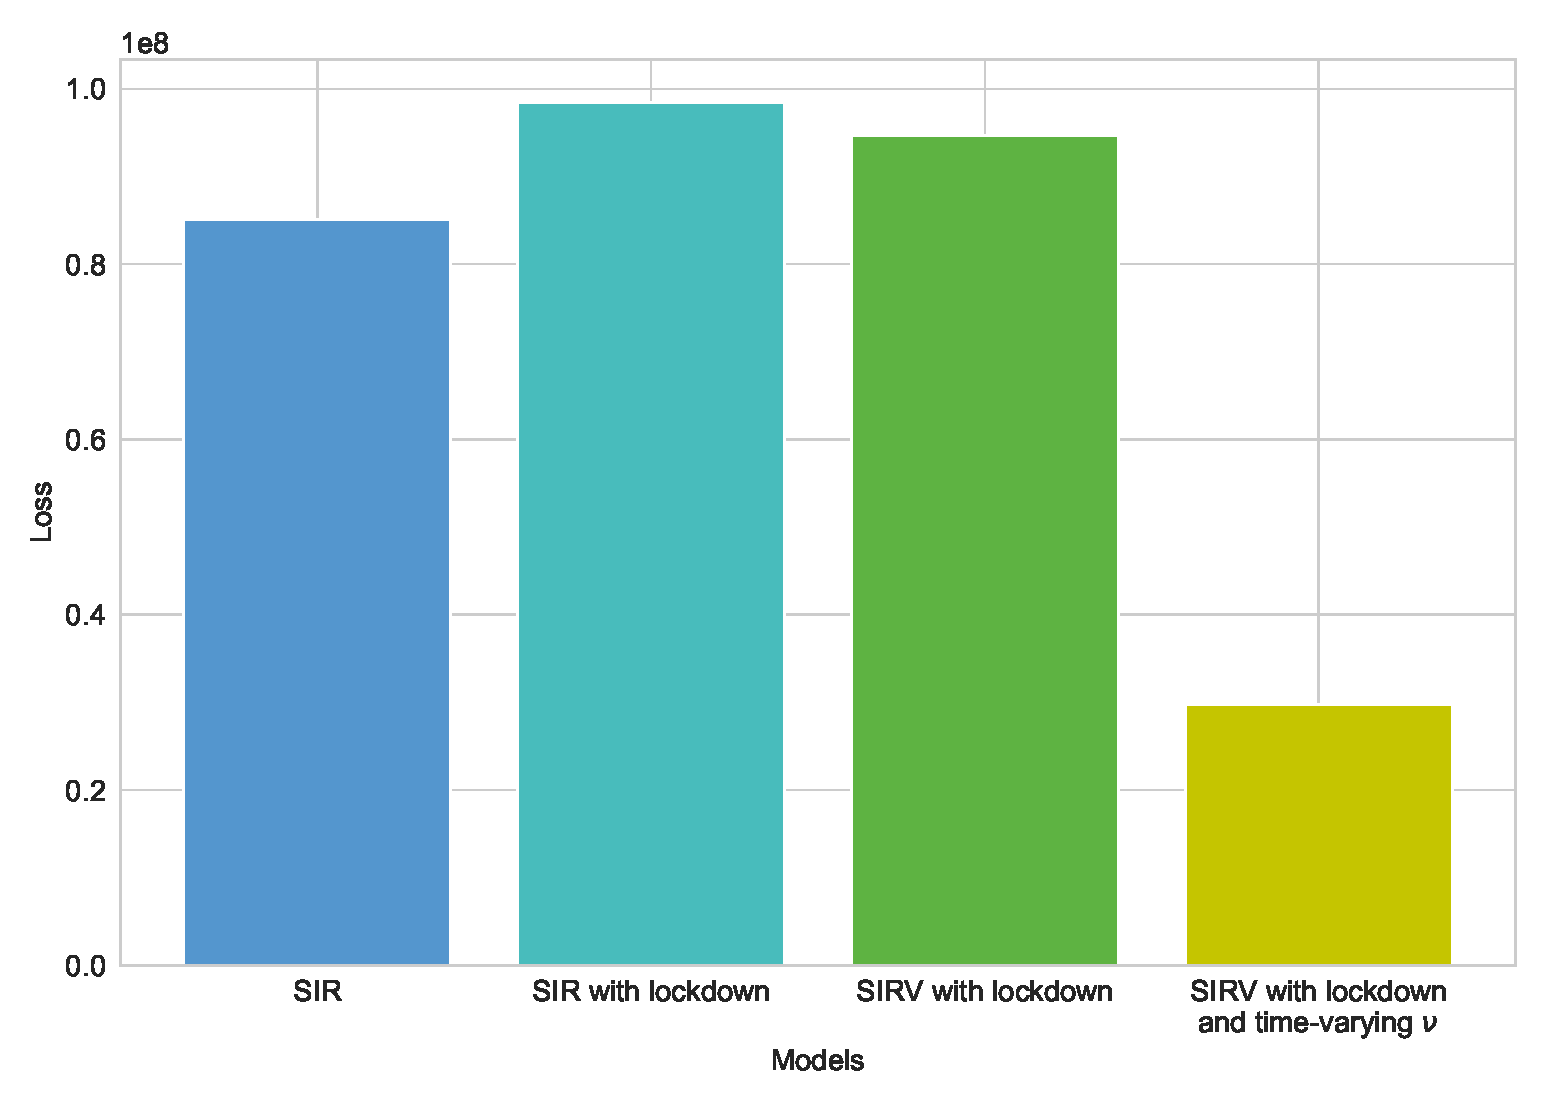
\includegraphics[width=\linewidth]{images/comparing_costs_IND.eps}
  \label{fig:comparing_costs_IND}
\end{figure}

With a time-varying $\nu$ (vaccination rate) and the effect of lockdown, our model is able to account for the infected individuals and reduce the cost in comparison to all the previously formalized models for the data. This shows how interventions and changes in the way people behave in response of a epidemic \cite{Caldwell2021} play a major role in the way the epidemic unfolds.

However, Non-pharmaceutical Interventions (NPIs) come with costs for developing nations. Below are scatter plots with pearson correlation, for three countries (India, Mexico, Brazil) which are Emerging Market and Developing Economies~\cite{IMFCovid} from May, 2020 to October, 2022.

\begin{figure}[H]
  \centering
  \caption{Stringency and GDP for Developing Economies}
  \begin{subfigure}[t]{0.48\textwidth}
    \centering
    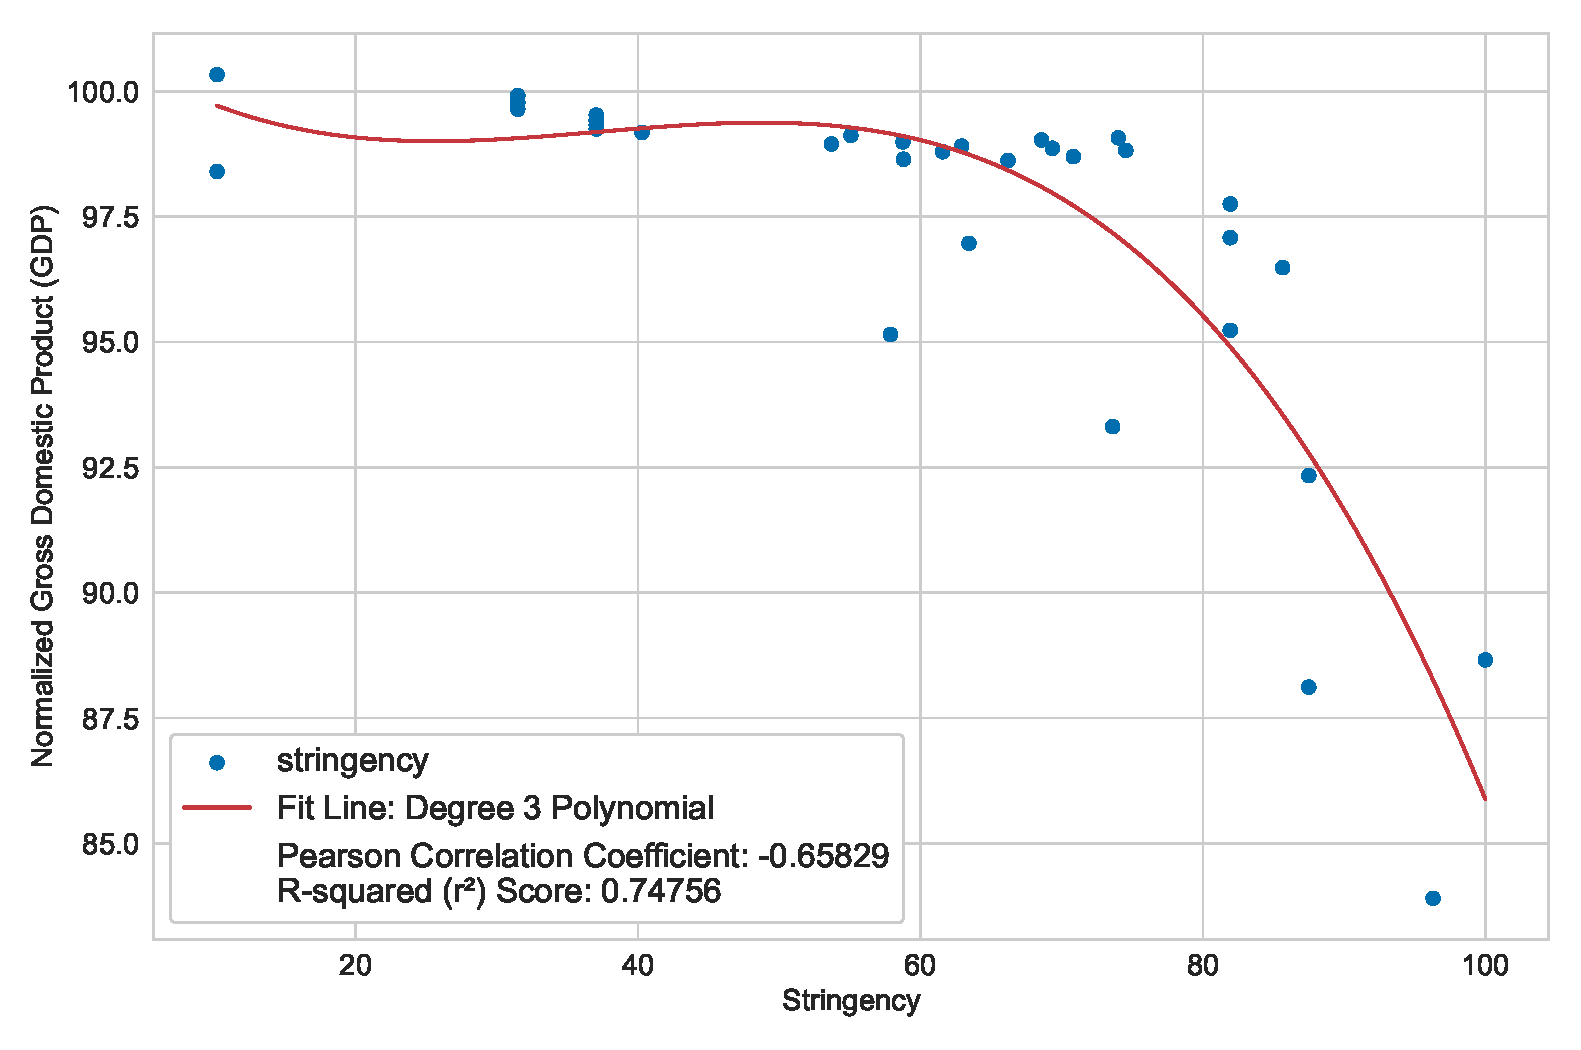
\includegraphics[width=\linewidth]{images/stringency_vs_gdp_IND.eps}
    \caption{Stringency and Normalized GDP for India}
  \end{subfigure}
  \label{fig:stringency_vs_gdp_IND}
  \hfill
  \begin{subfigure}[t]{0.48\textwidth}
    \centering
    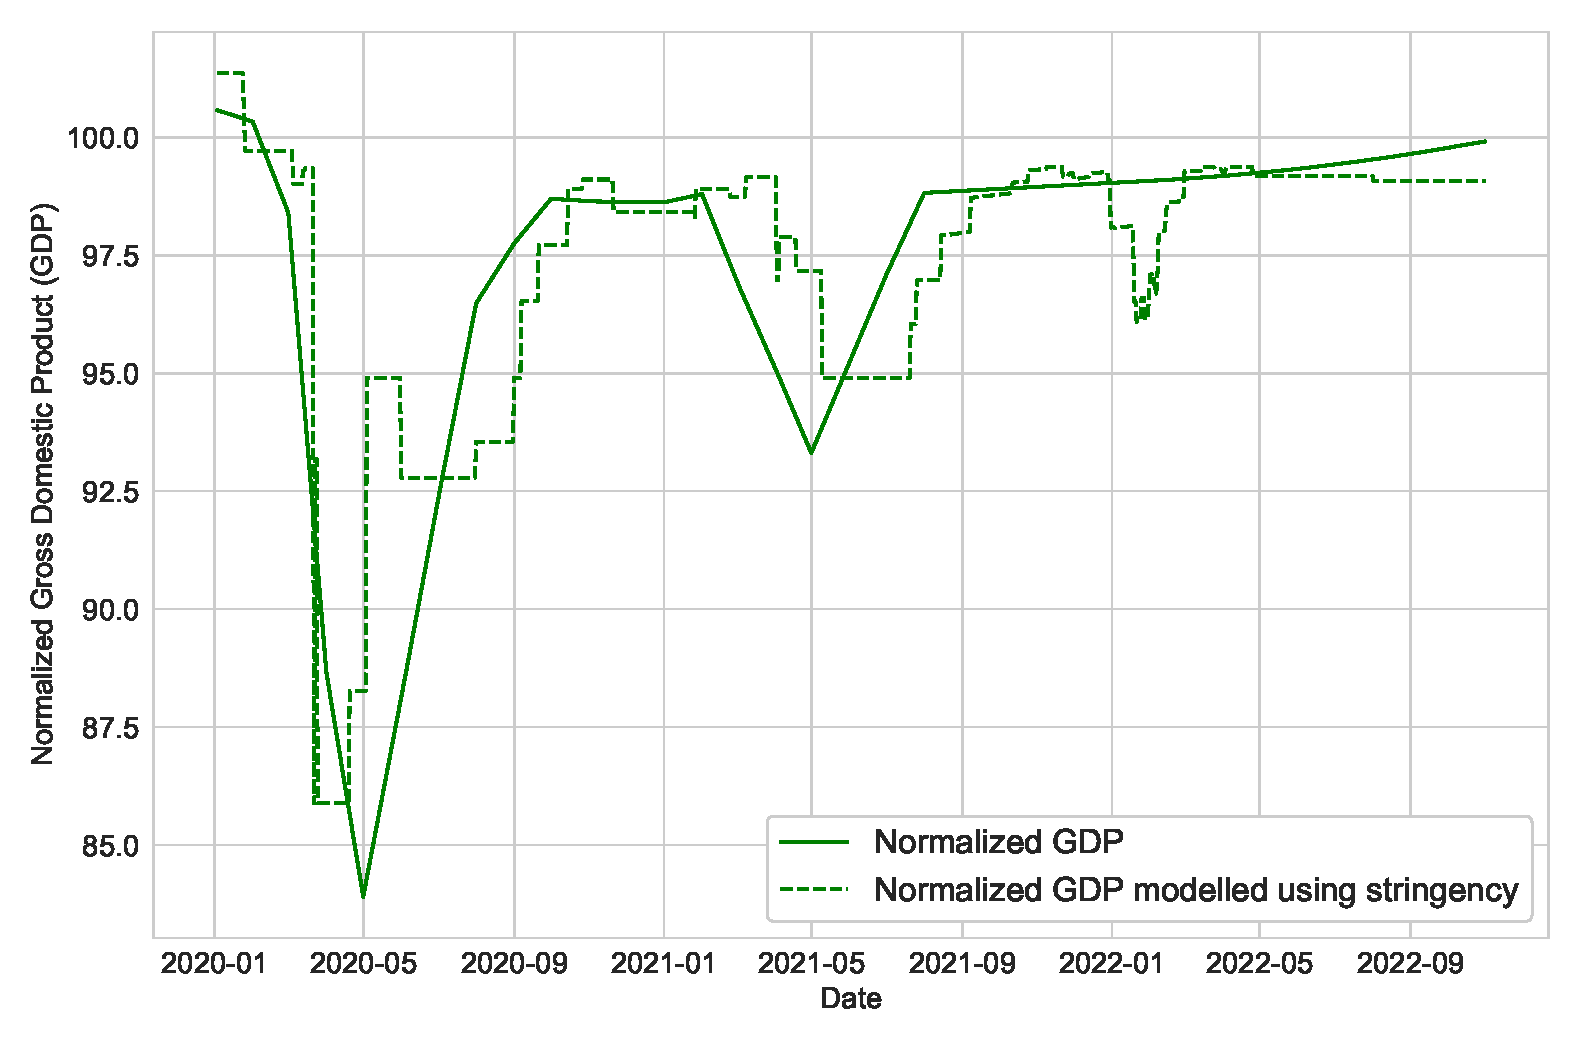
\includegraphics[width=\linewidth]{images/gdp_modelled_with_stringency_IND.eps}
    \caption{Normalized GDP modelled with Stringency for India}
  \end{subfigure}
  \label{fig:gdp_modelled_with_stringency_IND}

  \begin{subfigure}[t]{0.48\textwidth}
    \centering
    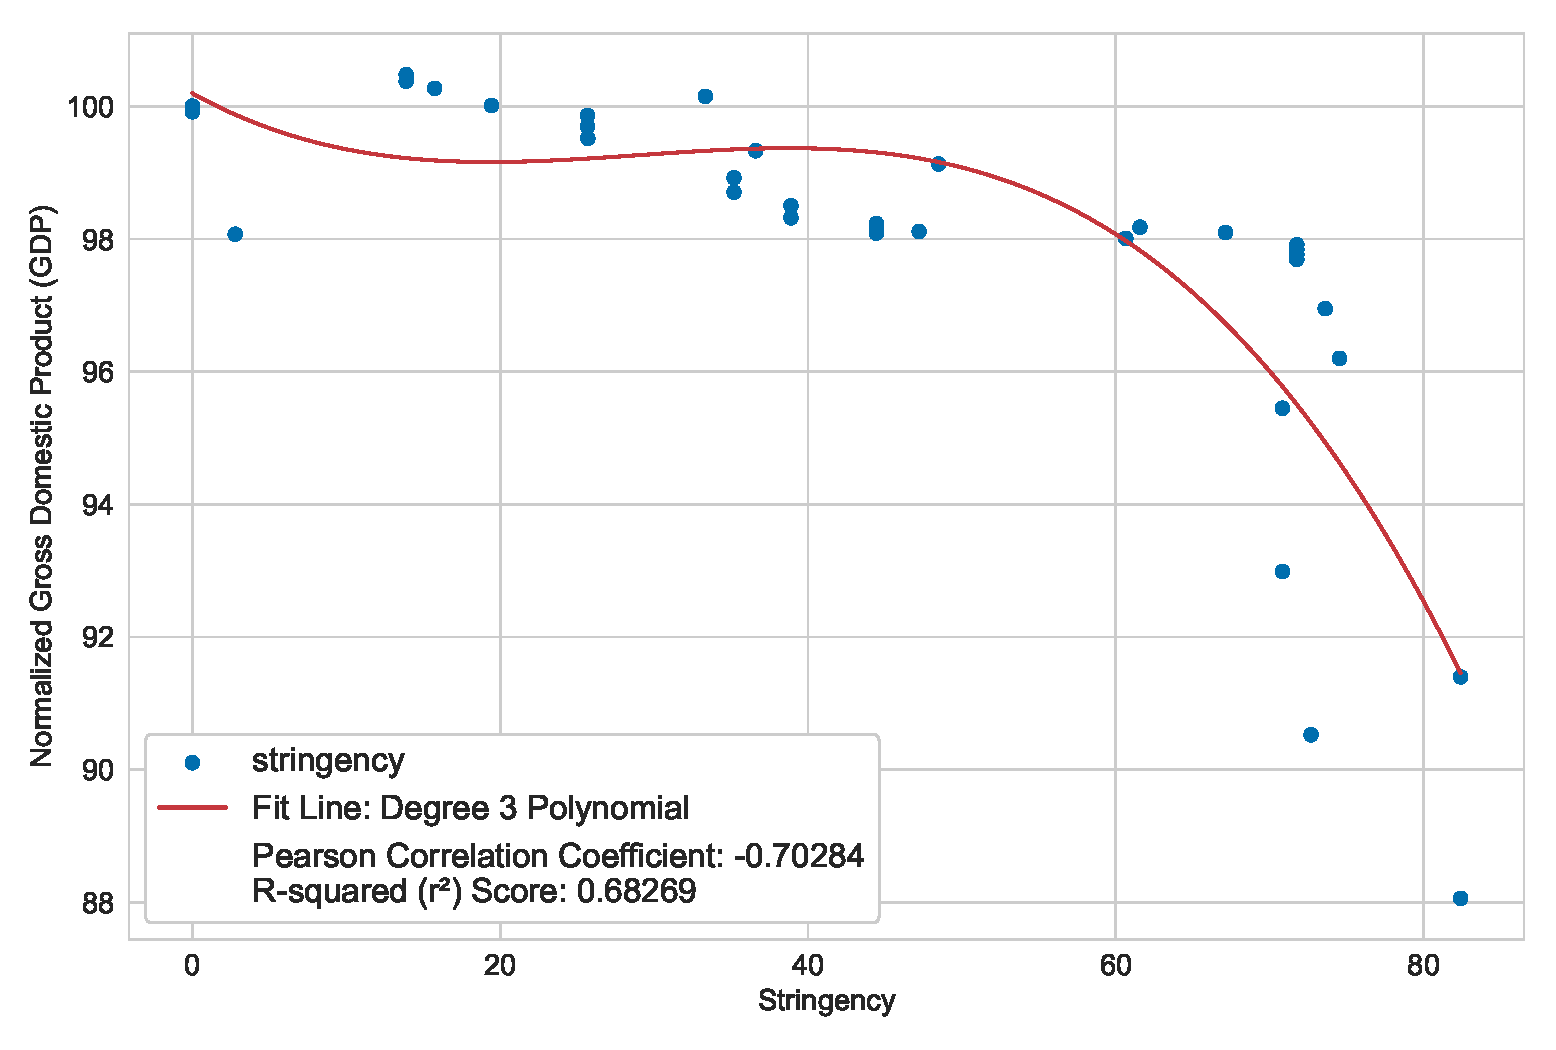
\includegraphics[width=\linewidth]{images/stringency_vs_gdp_MEX.eps}
    \caption{Stringency and Normalized GDP for Mexico}
  \end{subfigure}
  \label{fig:stringency_vs_gdp_MEX}
  \hfill
  \begin{subfigure}[t]{0.48\textwidth}
    \centering
    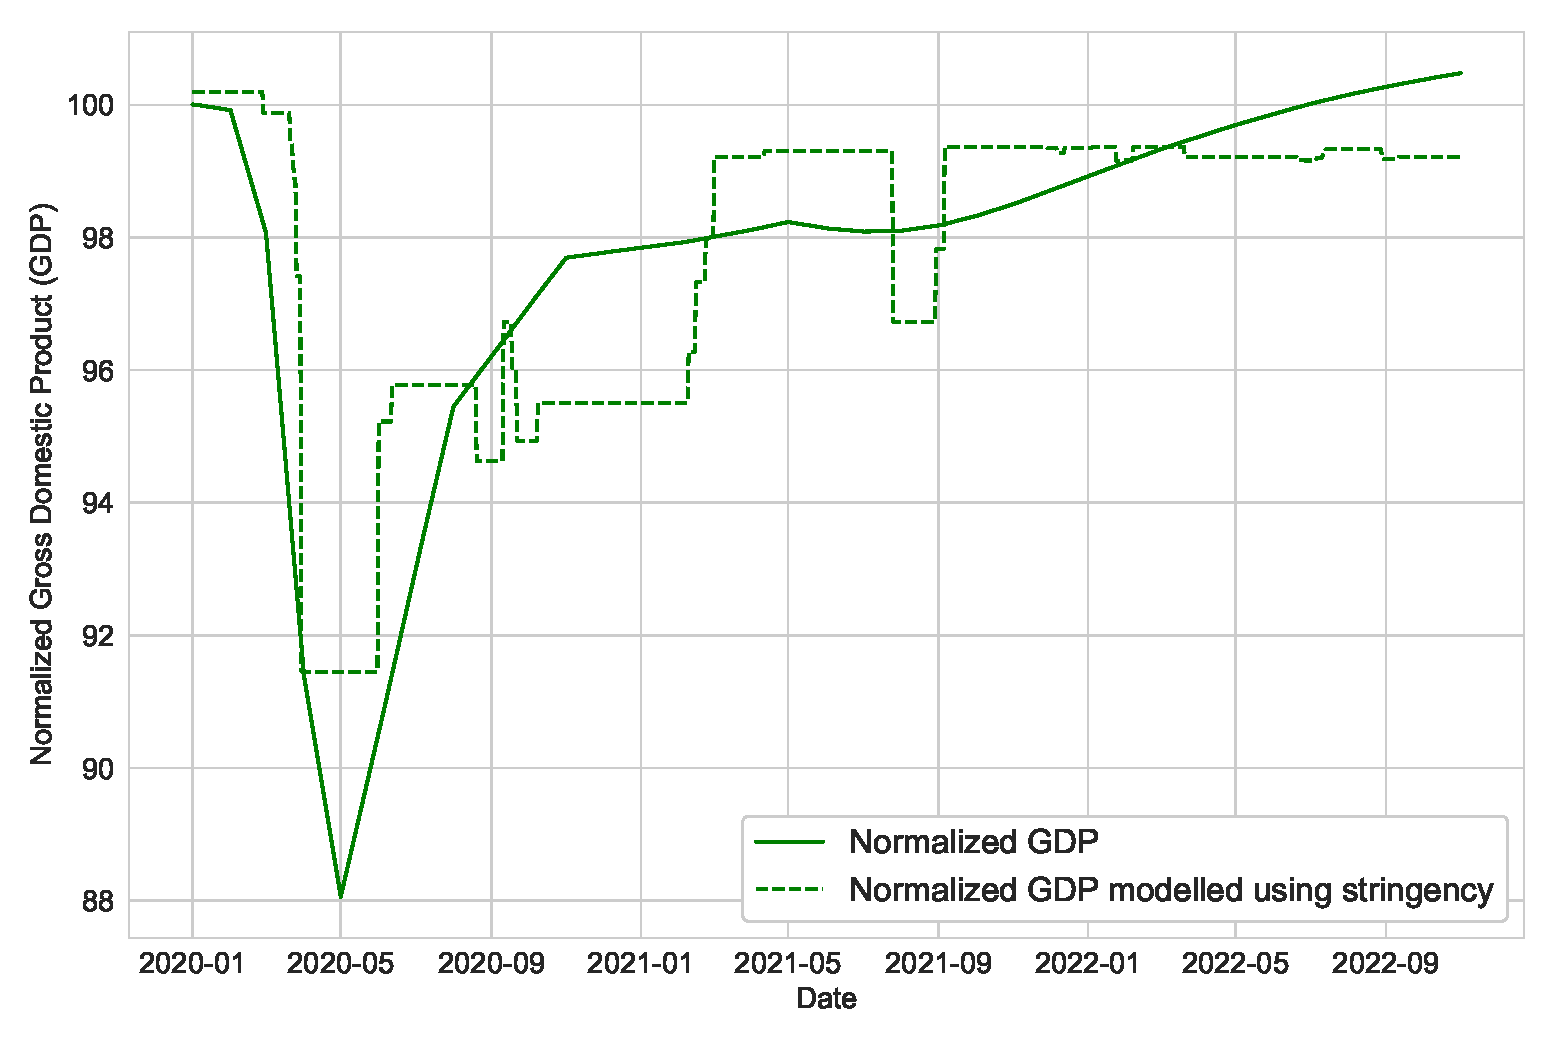
\includegraphics[width=\linewidth]{images/gdp_modelled_with_stringency_MEX.eps}
    \caption{Normalized GDP modelled with Stringency for Mexico}
  \end{subfigure}
  \label{fig:gdp_modelled_with_stringency_MEX}

  \begin{subfigure}[t]{0.48\textwidth}
    \centering
    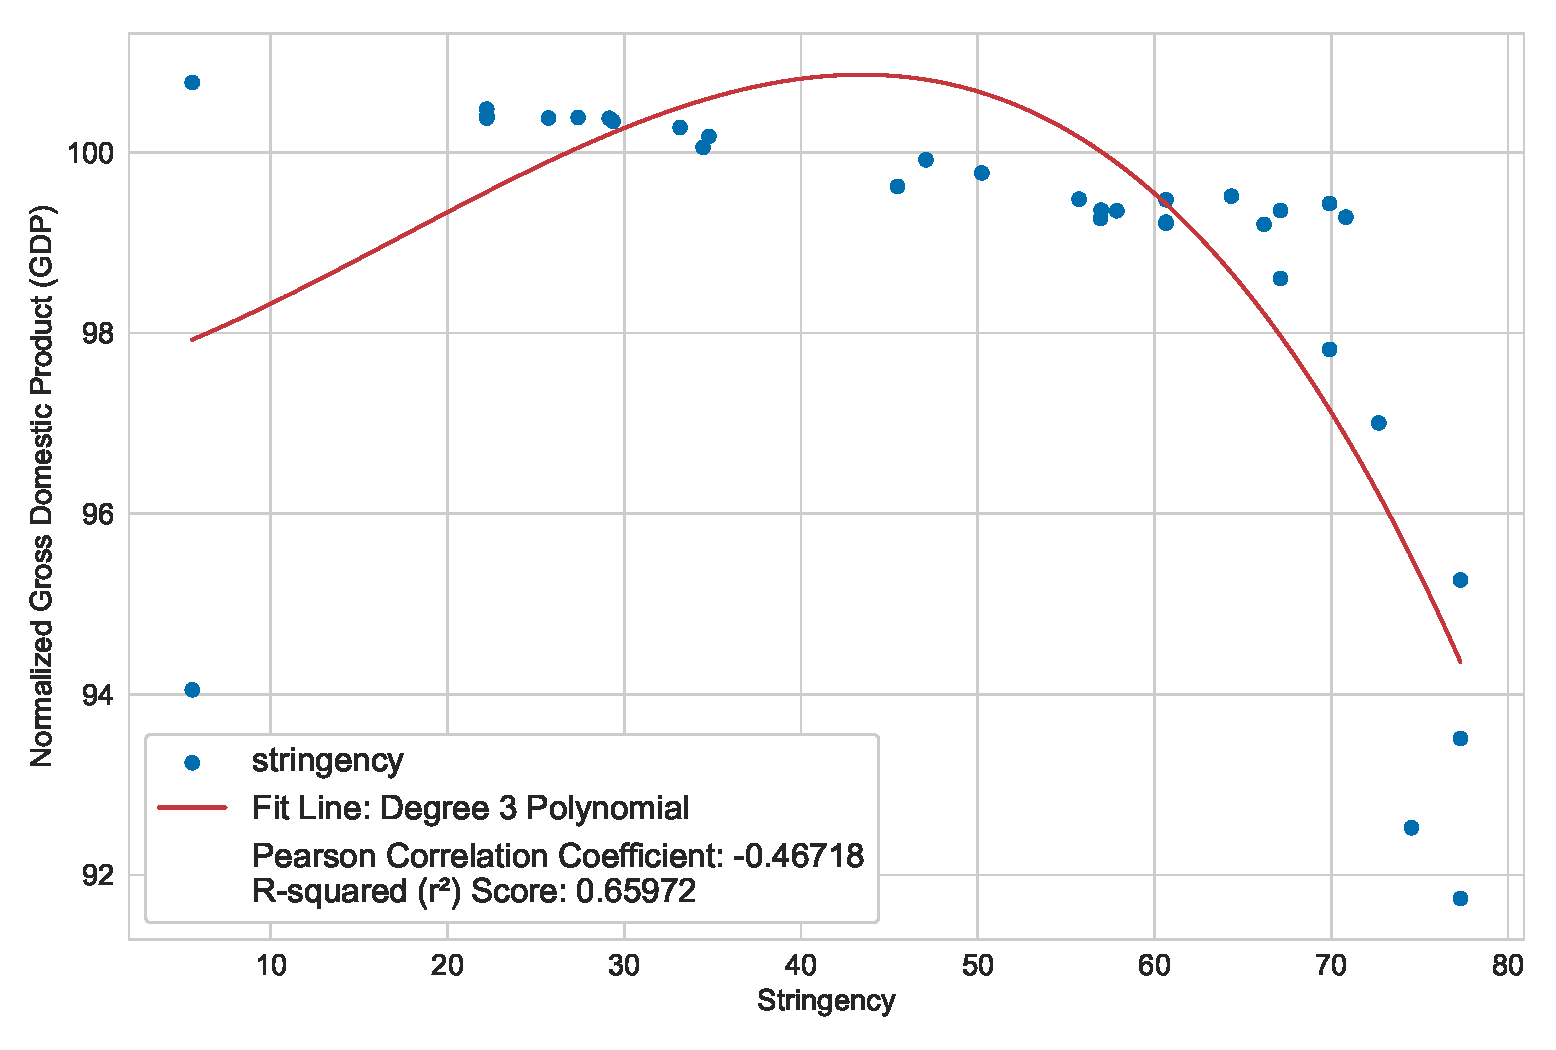
\includegraphics[width=\linewidth]{images/stringency_vs_gdp_BRA.eps}
    \caption{Stringency and Normalized GDP for Brazil}
  \end{subfigure}
  \label{fig:stringency_vs_gdp_BRA}
  \hfill
  \begin{subfigure}[t]{0.48\textwidth}
    \centering
    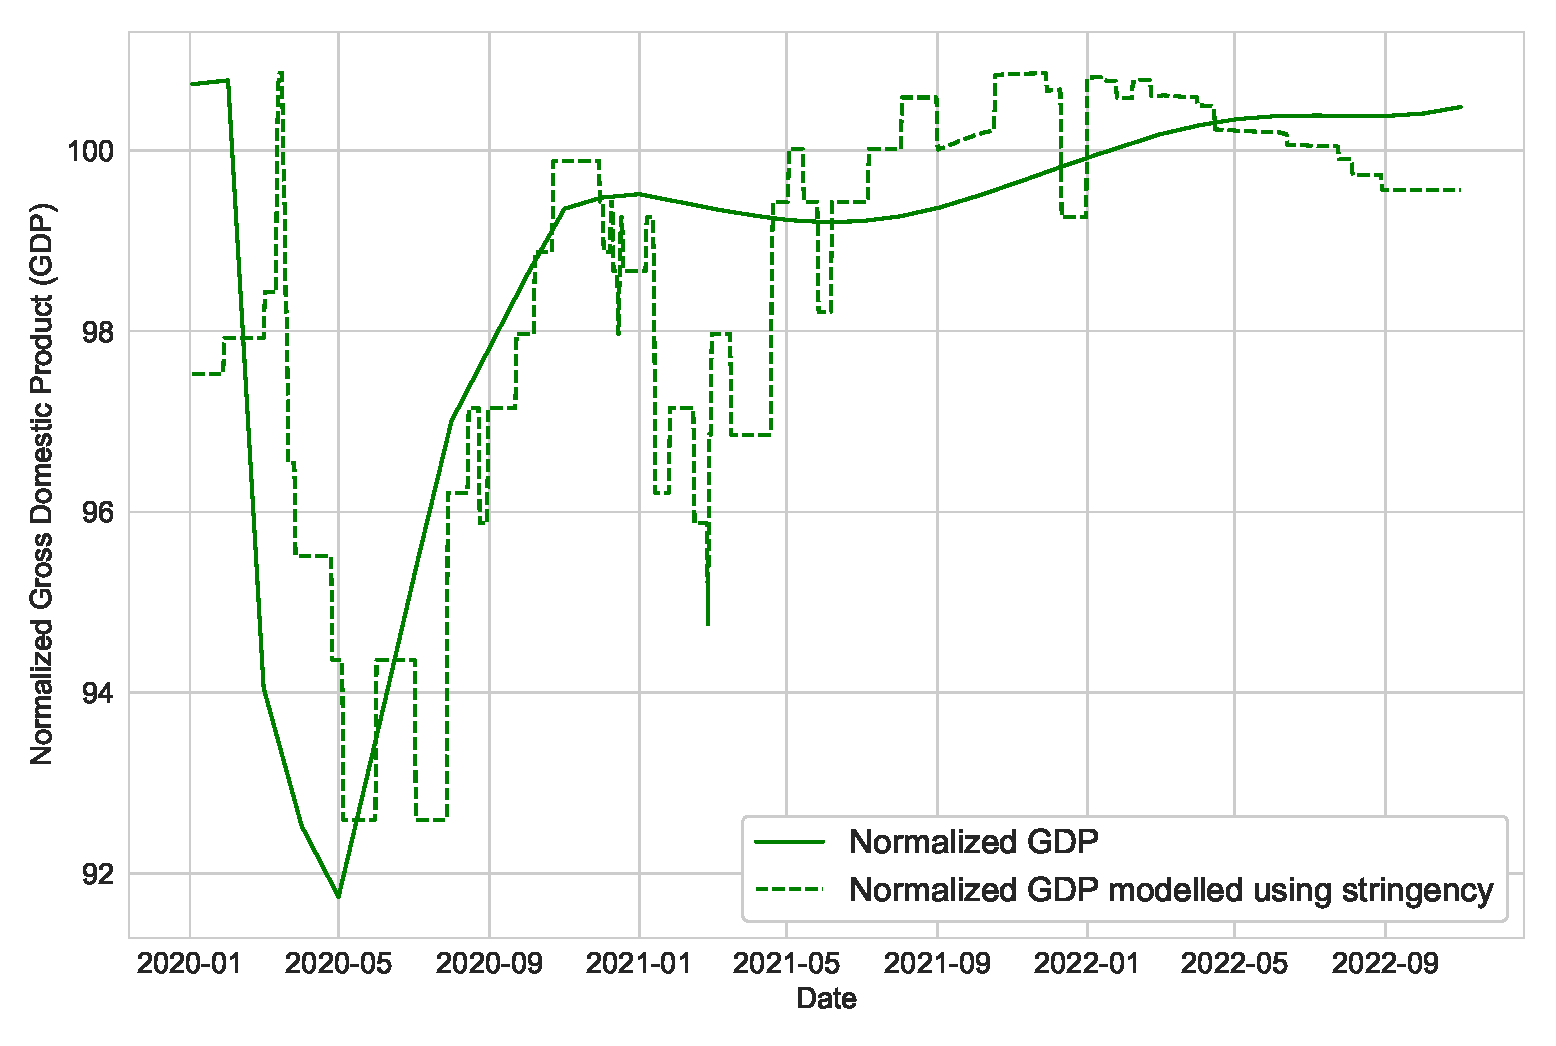
\includegraphics[width=\linewidth]{images/gdp_modelled_with_stringency_BRA.eps}
    \caption{Normalized GDP modelled with Stringency for Brazil}
  \end{subfigure}
  \label{fig:gdp_modelled_with_stringency_BRA}
\end{figure}

It can be observed that stringency has a negative impact on the normalized Gross domestic product (GDP). Therefore, in some countries policies made during an epidemic have competing costs. This is not the case for Advanced Economies like (USA, Japan, Canada).

\begin{figure}[H]
  \centering
  \caption{Stringency and GDP for Advanced Economies}
  \begin{subfigure}[t]{0.48\textwidth}
    \centering
    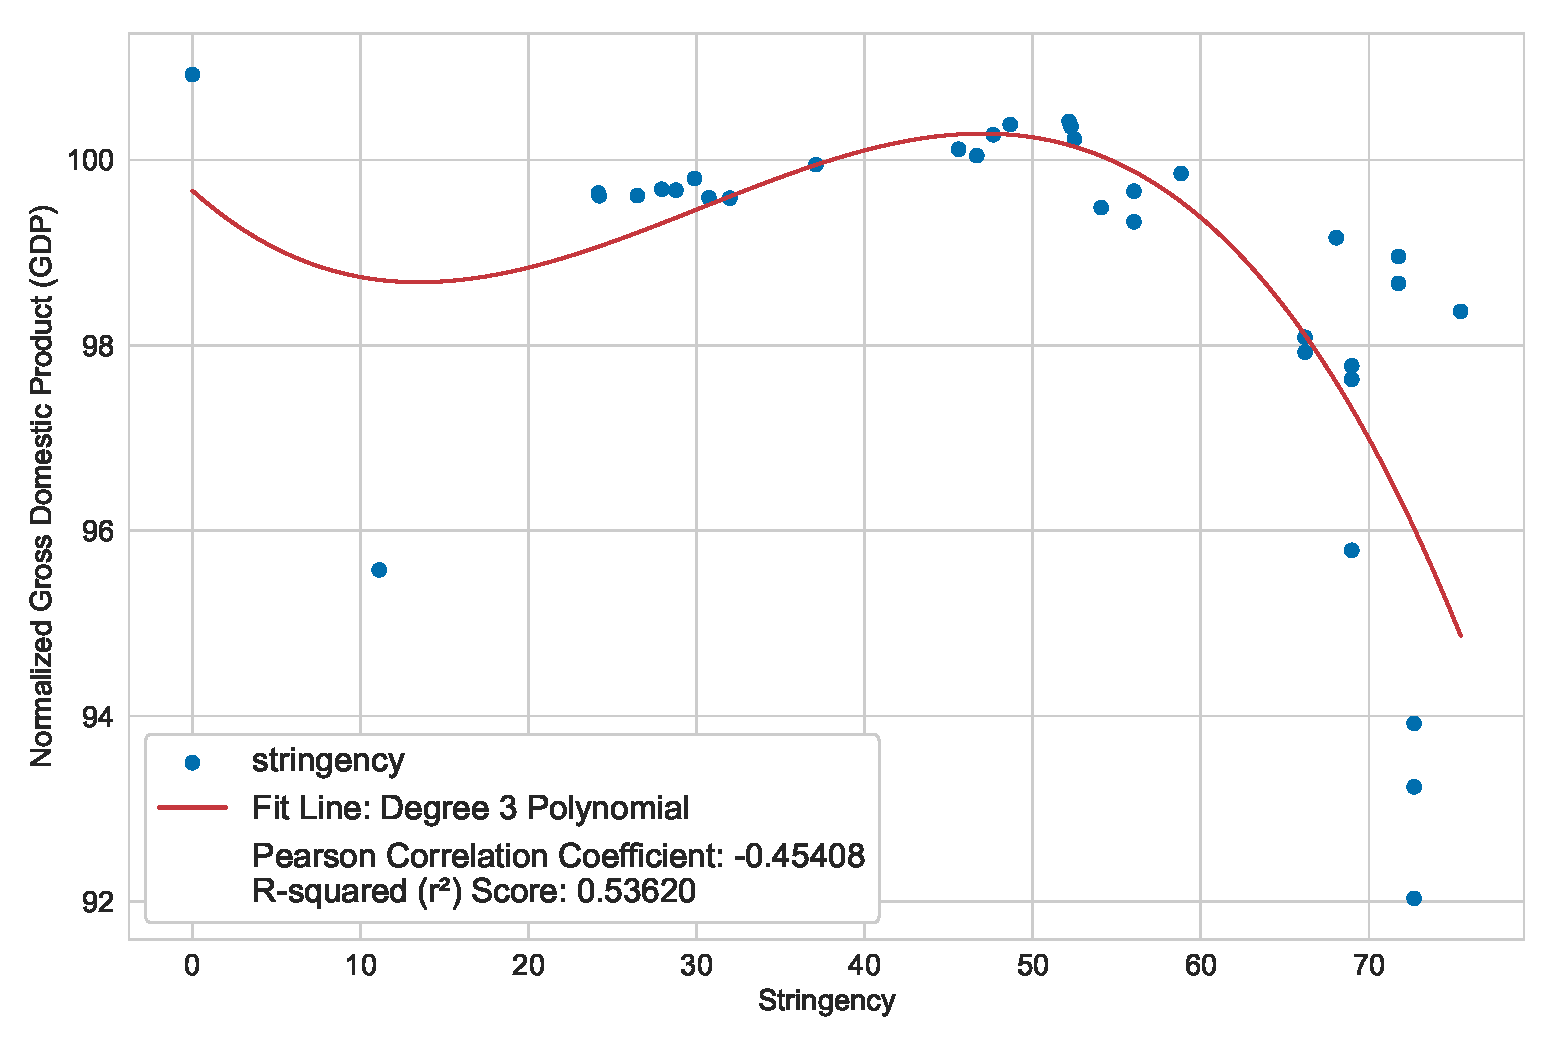
\includegraphics[width=\linewidth]{images/stringency_vs_gdp_USA.eps}
    \caption{Stringency and Normalized GDP for United States}
  \end{subfigure}
  \label{fig:stringency_vs_gdp_USA}
  \hfill
  \begin{subfigure}[t]{0.48\textwidth}
    \centering
    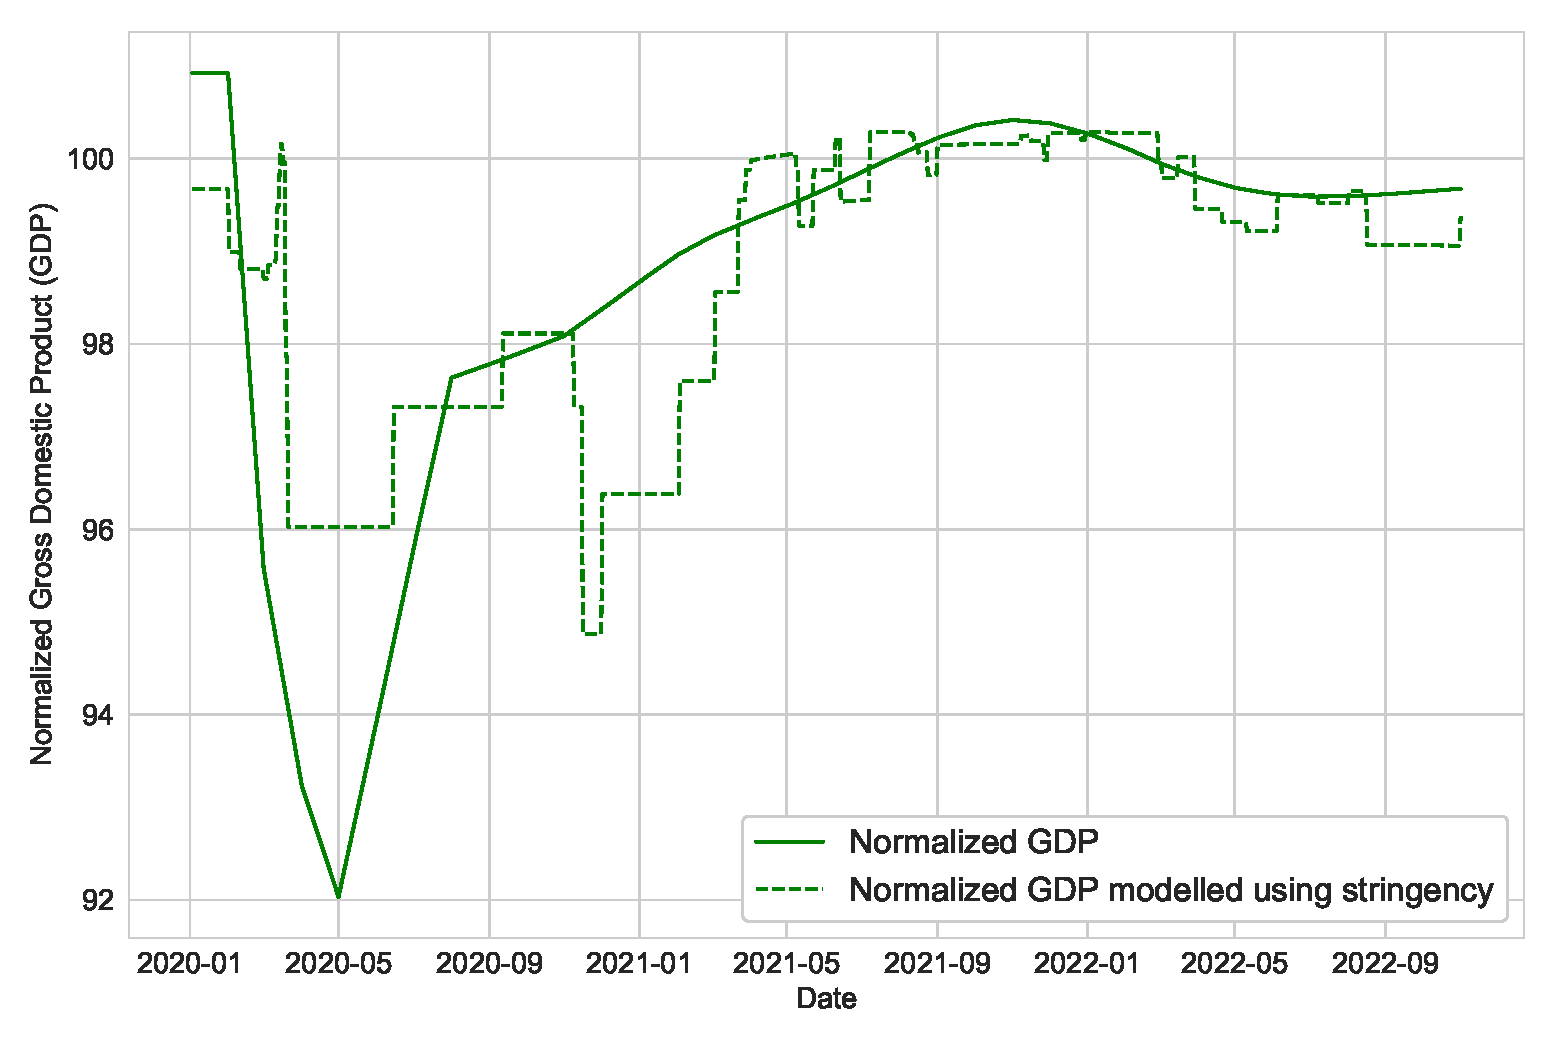
\includegraphics[width=\linewidth]{images/gdp_modelled_with_stringency_USA.eps}
    \caption{Normalized GDP modelled with Stringency for United States}
  \end{subfigure}
  \label{fig:gdp_modelled_with_stringency_USA}

  \begin{subfigure}[t]{0.48\textwidth}
    \centering
    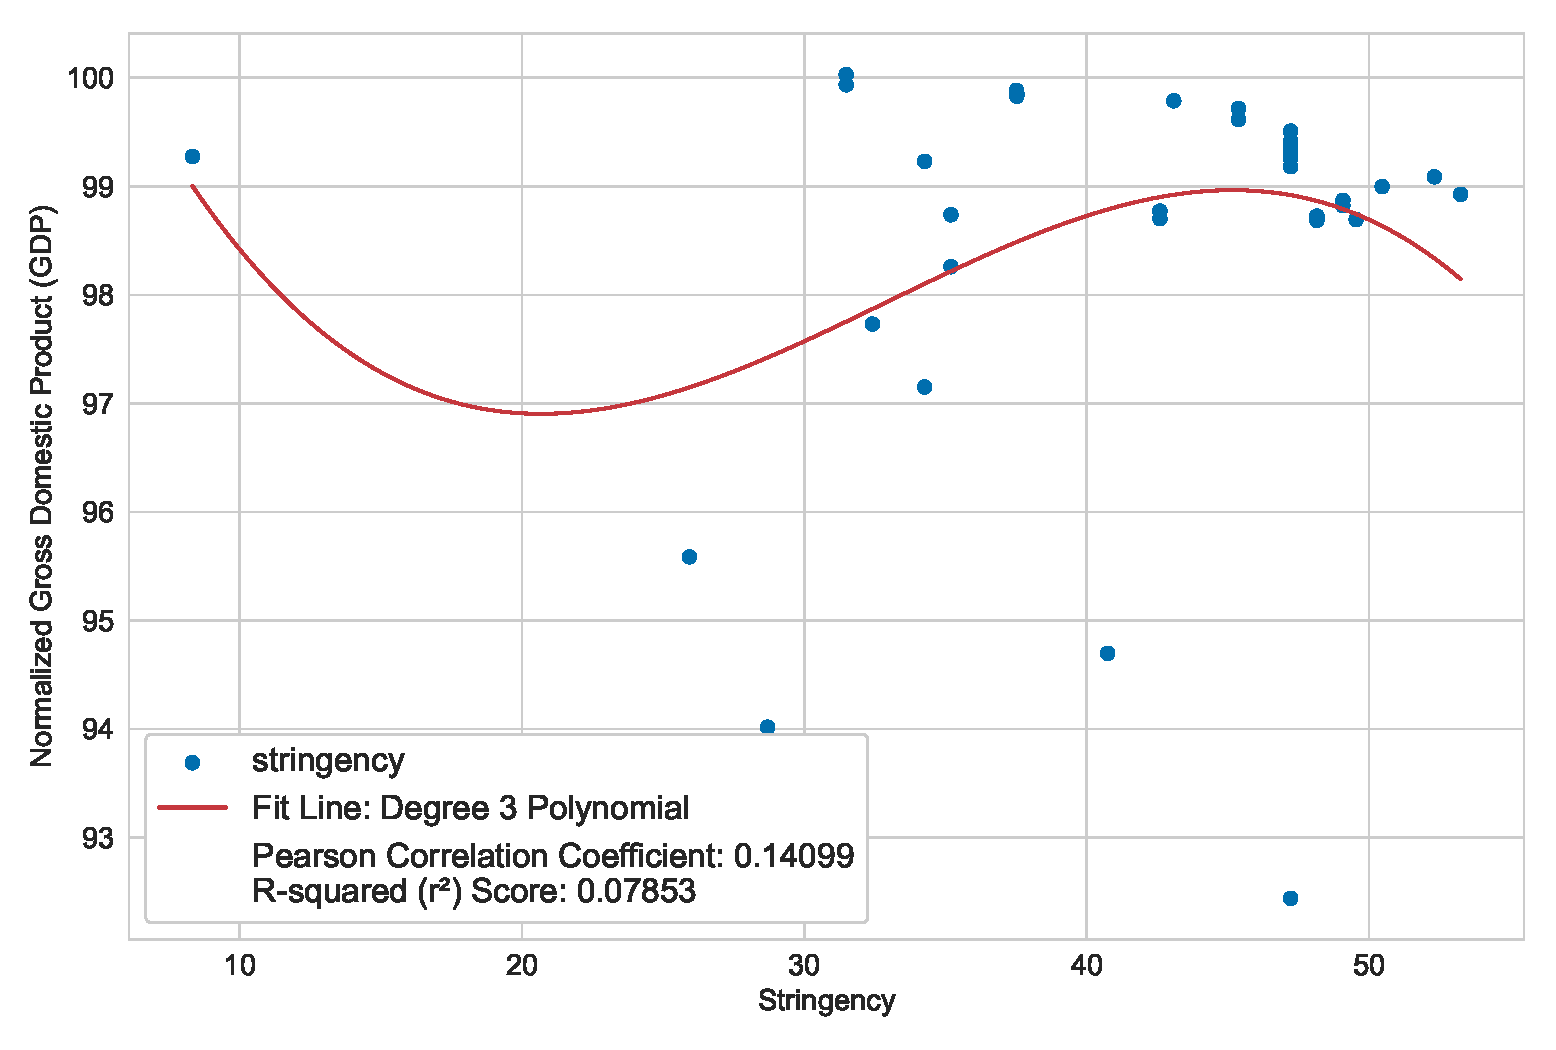
\includegraphics[width=\linewidth]{images/stringency_vs_gdp_JPN.eps}
    \caption{Stringency and Normalized GDP for Japan}
  \end{subfigure}
  \label{fig:stringency_vs_gdp_JPN}
  \hfill
  \begin{subfigure}[t]{0.48\textwidth}
    \centering
    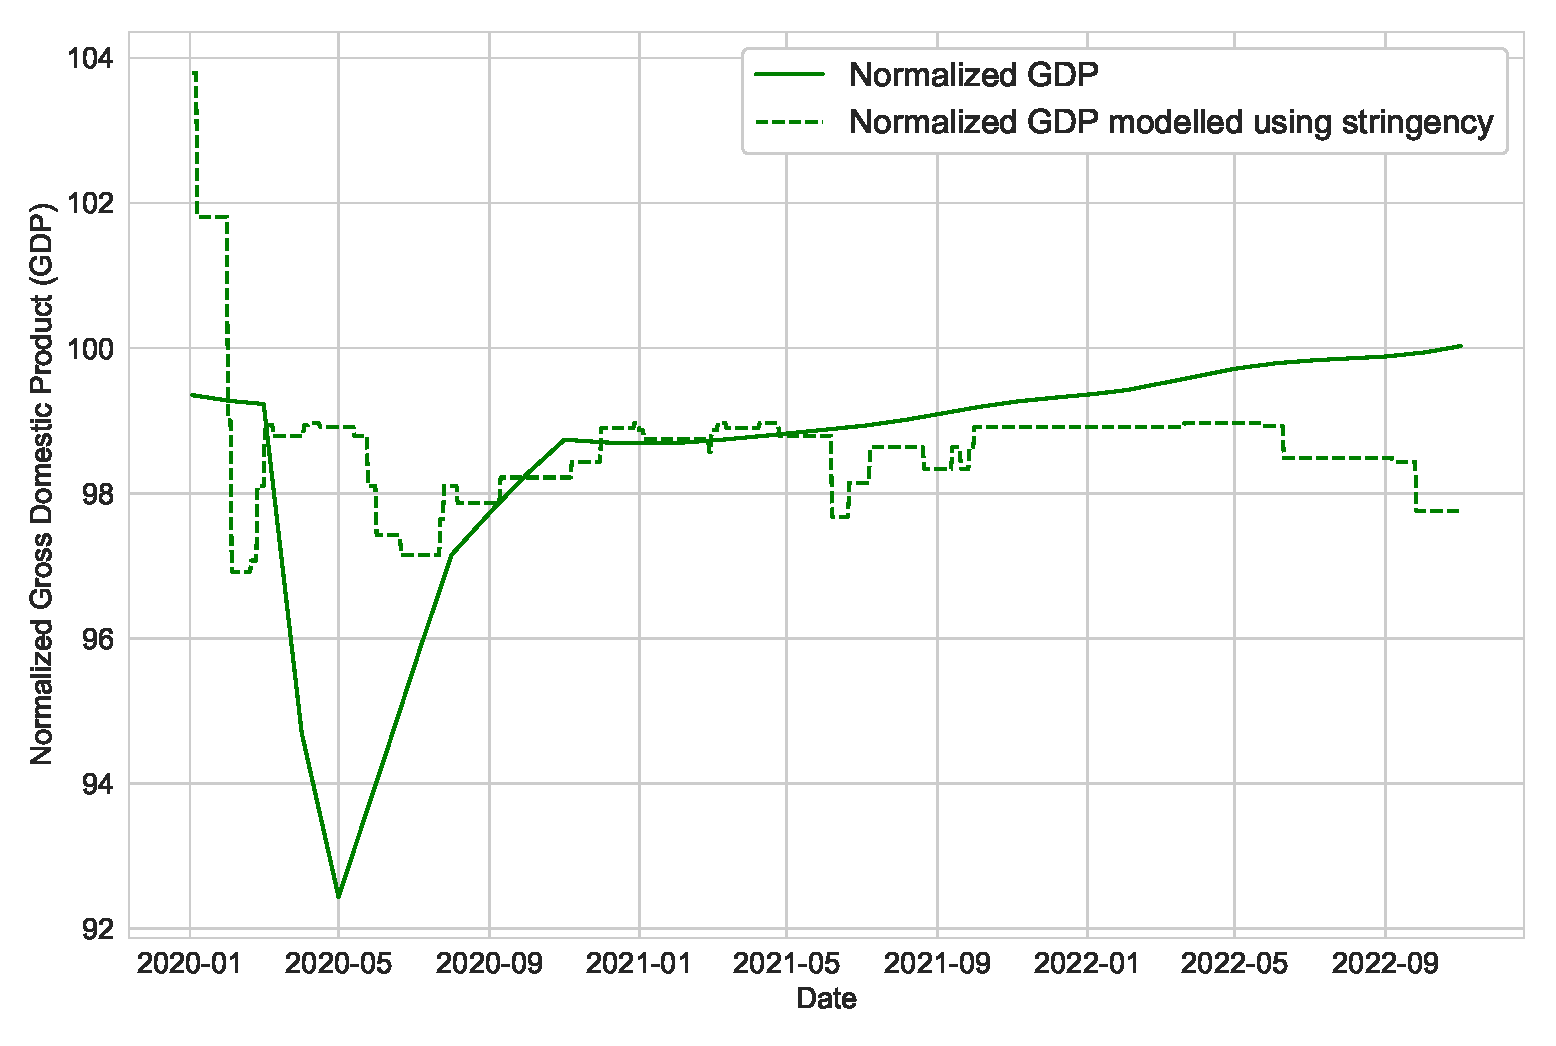
\includegraphics[width=\linewidth]{images/gdp_modelled_with_stringency_JPN.eps}
    \caption{Normalized GDP modelled with Stringency for Japan}
  \end{subfigure}
  \label{fig:gdp_modelled_with_stringency_JPN}

  \begin{subfigure}[t]{0.48\textwidth}
    \centering
    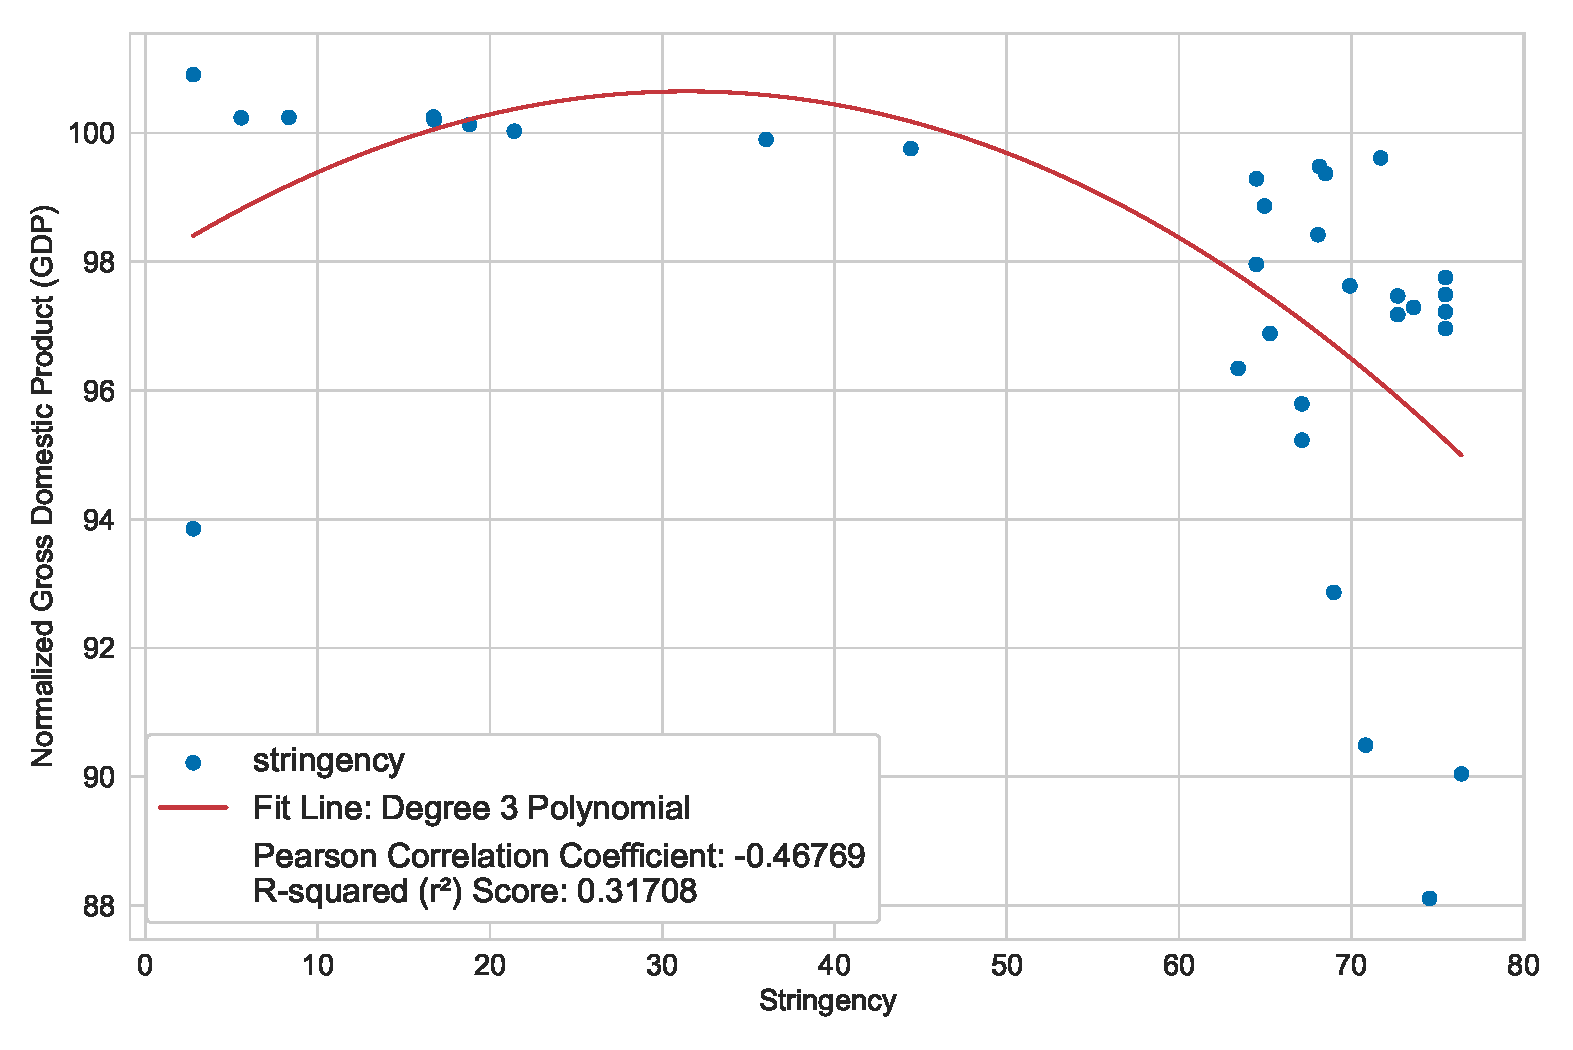
\includegraphics[width=\linewidth]{images/stringency_vs_gdp_CAN.eps}
    \caption{Stringency and Normalized GDP for Canada}
  \end{subfigure}
  \label{fig:stringency_vs_gdp_CAN}
  \hfill
  \begin{subfigure}[t]{0.48\textwidth}
    \centering
    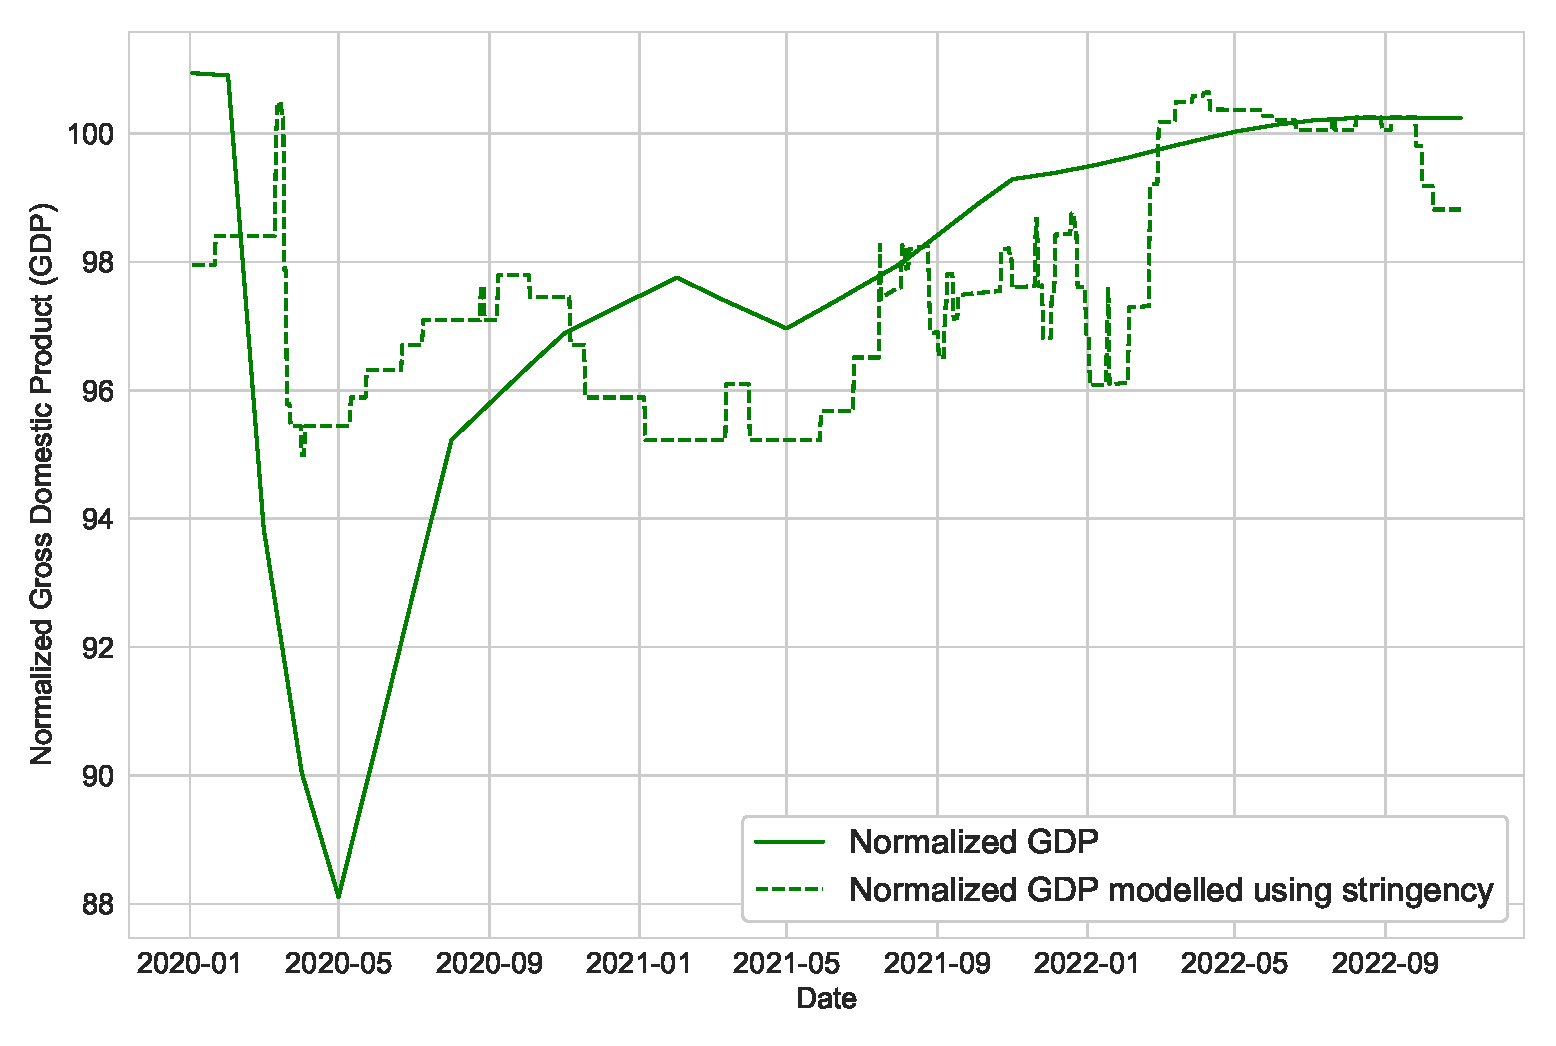
\includegraphics[width=\linewidth]{images/gdp_modelled_with_stringency_CAN.eps}
    \caption{Normalized GDP modelled with Stringency for Canada}
  \end{subfigure}
  \label{fig:gdp_modelled_with_stringency_CAN}
\end{figure}


\subsection*{Discussion}
The paper seeks to inspire epidemiologists by highlighting the advancements achieved through the application of reinforcement learning in policy making during the pandemic. We introduce a virtual environment that closely simulates a pandemic scenario and thoroughly explore innovative strategies for disease mitigation using reinforcement learning. Our proposed approach demonstrates compelling efficacy in achieving optimal decision-making, effectively balancing the formidable challenges posed by the pandemic and economic considerations. We are confident that this research contribution will forge a connection between epidemic studies and reinforcement learning, offering valuable insights to help humanity better defend against the ongoing pandemic crisis.

\subsection*{Experiment Settings}
\subsection{Dataset}
The population-level epidemiological data can be obtained from the 'Our World In Data COVID-19' dataset: \url{https://ourworldindata.org/coronavirus} or more specifically: \url{https://github.com/owid/covid-19-data/blob/master/public/data/owid-covid-data.csv}~\cite{owidcoronavirus}. Quaterly GDP data can be obtained from the 'Organisation for Economic Co-operation and Development': \url{https://www.oecd-ilibrary.org/economics/data/main-economic-indicators/main-economic-indicators-complete-database_data-00052-en}~\cite{economic_indicators_data}.

\subsection{Code}
We used stable-baseline3~\cite{JMLR:v22:20-1364}, Pytorch~\cite{paszke2019pytorch}, Scipy~\cite{Virtanen_2020}, Pandas, Matplotlib, Python~\cite{ScientificPython}.
Code: \url{https://github.com/psymbio/sir_rl}
% \bibliographystyle{plain}
\bibliography{sample}
\end{document}